\documentclass[1p]{elsarticle_modified}
%\bibliographystyle{elsarticle-num}

%\usepackage[colorlinks]{hyperref}
%\usepackage{abbrmath_seonhwa} %\Abb, \Ascr, \Acal ,\Abf, \Afrak
\usepackage{amsfonts}
\usepackage{amssymb}
\usepackage{amsmath}
\usepackage{amsthm}
\usepackage{scalefnt}
\usepackage{amsbsy}
\usepackage{kotex}
\usepackage{caption}
\usepackage{subfig}
\usepackage{color}
\usepackage{graphicx}
\usepackage{xcolor} %% white, black, red, green, blue, cyan, magenta, yellow
\usepackage{float}
\usepackage{setspace}
\usepackage{hyperref}

\usepackage{tikz}
\usetikzlibrary{arrows}

\usepackage{multirow}
\usepackage{array} % fixed length table
\usepackage{hhline}

%%%%%%%%%%%%%%%%%%%%%
\makeatletter
\renewcommand*\env@matrix[1][\arraystretch]{%
	\edef\arraystretch{#1}%
	\hskip -\arraycolsep
	\let\@ifnextchar\new@ifnextchar
	\array{*\c@MaxMatrixCols c}}
\makeatother %https://tex.stackexchange.com/questions/14071/how-can-i-increase-the-line-spacing-in-a-matrix
%%%%%%%%%%%%%%%

\usepackage[normalem]{ulem}

\newcommand{\msout}[1]{\ifmmode\text{\sout{\ensuremath{#1}}}\else\sout{#1}\fi}
%SOURCE: \msout is \stkout macro in https://tex.stackexchange.com/questions/20609/strikeout-in-math-mode

\newcommand{\cancel}[1]{
	\ifmmode
	{\color{red}\msout{#1}}
	\else
	{\color{red}\sout{#1}}
	\fi
}

\newcommand{\add}[1]{
	{\color{blue}\uwave{#1}}
}

\newcommand{\replace}[2]{
	\ifmmode
	{\color{red}\msout{#1}}{\color{blue}\uwave{#2}}
	\else
	{\color{red}\sout{#1}}{\color{blue}\uwave{#2}}
	\fi
}

\newcommand{\Sol}{\mathcal{S}} %segment
\newcommand{\D}{D} %diagram
\newcommand{\A}{\mathcal{A}} %arc


%%%%%%%%%%%%%%%%%%%%%%%%%%%%%5 test

\def\sl{\operatorname{\textup{SL}}(2,\Cbb)}
\def\psl{\operatorname{\textup{PSL}}(2,\Cbb)}
\def\quan{\mkern 1mu \triangleright \mkern 1mu}

\theoremstyle{definition}
\newtheorem{thm}{Theorem}[section]
\newtheorem{prop}[thm]{Proposition}
\newtheorem{lem}[thm]{Lemma}
\newtheorem{ques}[thm]{Question}
\newtheorem{cor}[thm]{Corollary}
\newtheorem{defn}[thm]{Definition}
\newtheorem{exam}[thm]{Example}
\newtheorem{rmk}[thm]{Remark}
\newtheorem{alg}[thm]{Algorithm}

\newcommand{\I}{\sqrt{-1}}
\begin{document}

%\begin{frontmatter}
%
%\title{Boundary parabolic representations of knots up to 8 crossings}
%
%%% Group authors per affiliation:
%\author{Yunhi Cho} 
%\address{Department of Mathematics, University of Seoul, Seoul, Korea}
%\ead{yhcho@uos.ac.kr}
%
%
%\author{Seonhwa Kim} %\fnref{s_kim}}
%\address{Center for Geometry and Physics, Institute for Basic Science, Pohang, 37673, Korea}
%\ead{ryeona17@ibs.re.kr}
%
%\author{Hyuk Kim}
%\address{Department of Mathematical Sciences, Seoul National University, Seoul 08826, Korea}
%\ead{hyukkim@snu.ac.kr}
%
%\author{Seokbeom Yoon}
%\address{Department of Mathematical Sciences, Seoul National University, Seoul, 08826,  Korea}
%\ead{sbyoon15@snu.ac.kr}
%
%\begin{abstract}
%We find all boundary parabolic representation of knots up to 8 crossings.
%
%\end{abstract}
%\begin{keyword}
%    \MSC[2010] 57M25 
%\end{keyword}
%
%\end{frontmatter}

%\linenumbers
%\tableofcontents
%
\newcommand\colored[1]{\textcolor{white}{\rule[-0.35ex]{0.8em}{1.4ex}}\kern-0.8em\color{red} #1}%
%\newcommand\colored[1]{\textcolor{white}{ #1}\kern-2.17ex	\textcolor{white}{ #1}\kern-1.81ex	\textcolor{white}{ #1}\kern-2.15ex\color{red}#1	}

{\Large $\underline{12a_{1113}~(K12a_{1113})}$}

\setlength{\tabcolsep}{10pt}
\renewcommand{\arraystretch}{1.6}
\vspace{1cm}\begin{tabular}{m{100pt}>{\centering\arraybackslash}m{274pt}}
\multirow{5}{120pt}{
	\centering
	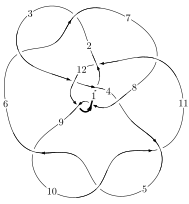
\includegraphics[width=112pt]{../../../GIT/diagram.site/Diagrams/png/1914_12a_1113.png}\\
\ \ \ A knot diagram\footnotemark}&
\allowdisplaybreaks
\textbf{Linearized knot diagam} \\
\cline{2-2}
 &
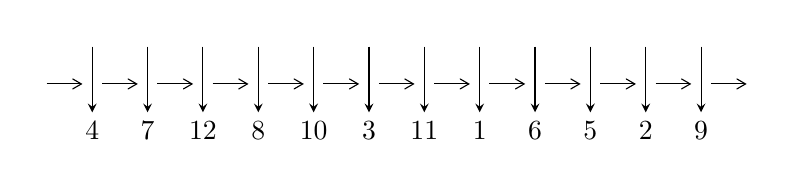
\begin{tikzpicture}[x=20pt, y=17pt]
	% nodes
	\node (C0) at (0, 0) {};
	\node (C1) at (1, 0) {};
	\node (C1U) at (1, +1) {};
	\node (C1D) at (1, -1) {4};

	\node (C2) at (2, 0) {};
	\node (C2U) at (2, +1) {};
	\node (C2D) at (2, -1) {7};

	\node (C3) at (3, 0) {};
	\node (C3U) at (3, +1) {};
	\node (C3D) at (3, -1) {12};

	\node (C4) at (4, 0) {};
	\node (C4U) at (4, +1) {};
	\node (C4D) at (4, -1) {8};

	\node (C5) at (5, 0) {};
	\node (C5U) at (5, +1) {};
	\node (C5D) at (5, -1) {10};

	\node (C6) at (6, 0) {};
	\node (C6U) at (6, +1) {};
	\node (C6D) at (6, -1) {3};

	\node (C7) at (7, 0) {};
	\node (C7U) at (7, +1) {};
	\node (C7D) at (7, -1) {11};

	\node (C8) at (8, 0) {};
	\node (C8U) at (8, +1) {};
	\node (C8D) at (8, -1) {1};

	\node (C9) at (9, 0) {};
	\node (C9U) at (9, +1) {};
	\node (C9D) at (9, -1) {6};

	\node (C10) at (10, 0) {};
	\node (C10U) at (10, +1) {};
	\node (C10D) at (10, -1) {5};

	\node (C11) at (11, 0) {};
	\node (C11U) at (11, +1) {};
	\node (C11D) at (11, -1) {2};

	\node (C12) at (12, 0) {};
	\node (C12U) at (12, +1) {};
	\node (C12D) at (12, -1) {9};
	\node (C13) at (13, 0) {};

	% arrows
	\draw[->,>={angle 60}]
	(C0) edge (C1) (C1) edge (C2) (C2) edge (C3) (C3) edge (C4) (C4) edge (C5) (C5) edge (C6) (C6) edge (C7) (C7) edge (C8) (C8) edge (C9) (C9) edge (C10) (C10) edge (C11) (C11) edge (C12) (C12) edge (C13) ;	\draw[->,>=stealth]
	(C1U) edge (C1D) (C2U) edge (C2D) (C3U) edge (C3D) (C4U) edge (C4D) (C5U) edge (C5D) (C6U) edge (C6D) (C7U) edge (C7D) (C8U) edge (C8D) (C9U) edge (C9D) (C10U) edge (C10D) (C11U) edge (C11D) (C12U) edge (C12D) ;
	\end{tikzpicture} \\
\hhline{~~} \\& 
\textbf{Solving Sequence} \\ \cline{2-2} 
 &
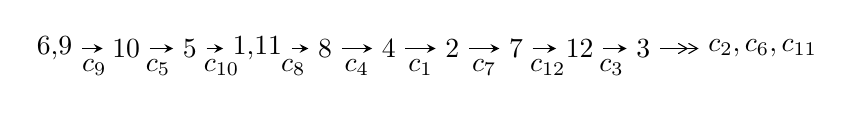
\begin{tikzpicture}[x=23pt, y=7pt]
	% node
	\node (A0) at (-1/8, 0) {6,9};
	\node (A1) at (1, 0) {10};
	\node (A2) at (2, 0) {5};
	\node (A3) at (49/16, 0) {1,11};
	\node (A4) at (33/8, 0) {8};
	\node (A5) at (41/8, 0) {4};
	\node (A6) at (49/8, 0) {2};
	\node (A7) at (57/8, 0) {7};
	\node (A8) at (65/8, 0) {12};
	\node (A9) at (73/8, 0) {3};
	\node (C1) at (1/2, -1) {$c_{9}$};
	\node (C2) at (3/2, -1) {$c_{5}$};
	\node (C3) at (5/2, -1) {$c_{10}$};
	\node (C4) at (29/8, -1) {$c_{8}$};
	\node (C5) at (37/8, -1) {$c_{4}$};
	\node (C6) at (45/8, -1) {$c_{1}$};
	\node (C7) at (53/8, -1) {$c_{7}$};
	\node (C8) at (61/8, -1) {$c_{12}$};
	\node (C9) at (69/8, -1) {$c_{3}$};
	\node (A10) at (11, 0) {$c_{2},c_{6},c_{11}$};

	% edge
	\draw[->,>=stealth]	
	(A0) edge (A1) (A1) edge (A2) (A2) edge (A3) (A3) edge (A4) (A4) edge (A5) (A5) edge (A6) (A6) edge (A7) (A7) edge (A8) (A8) edge (A9) ;
	\draw[->>,>={angle 60}]	
	(A9) edge (A10);
\end{tikzpicture} \\ 

\end{tabular} \\

\footnotetext{
The image of knot diagram is generated by the software ``\textbf{Draw programme}" developed by Andrew Bartholomew(\url{http://www.layer8.co.uk/maths/draw/index.htm\#Running-draw}), where we modified some parts for our purpose(\url{https://github.com/CATsTAILs/LinksPainter}).
}\phantom \\ \newline 
\centering \textbf{Ideals for irreducible components\footnotemark of $X_{\text{par}}$} 
 
\begin{align*}
I^u_{1}&=\langle 
2.32908\times10^{29} u^{40}+1.73331\times10^{30} u^{39}+\cdots+3.94562\times10^{29} b+4.96788\times10^{30},\\
\phantom{I^u_{1}}&\phantom{= \langle  }6.00345\times10^{29} u^{40}+4.26908\times10^{30} u^{39}+\cdots+1.97281\times10^{30} a-8.10812\times10^{30},\\
\phantom{I^u_{1}}&\phantom{= \langle  }u^{41}+8 u^{40}+\cdots+194 u+20\rangle \\
I^u_{2}&=\langle 
5.17859\times10^{49} a u^{52}-8.79765\times10^{49} u^{52}+\cdots+9.52947\times10^{49} a-3.28551\times10^{50},\\
\phantom{I^u_{2}}&\phantom{= \langle  }-1.62239\times10^{46} a u^{52}-9.06685\times10^{45} u^{52}+\cdots-7.15132\times10^{46} a+1.44688\times10^{46},\\
\phantom{I^u_{2}}&\phantom{= \langle  }u^{53}-3 u^{52}+\cdots+6 u-1\rangle \\
I^u_{3}&=\langle 
286 u^{15} a+870 u^{15}+\cdots+412 a-1440,\;u^{15} a-5 u^{15}+\cdots-2 a+3,\;u^{16}-2 u^{15}+\cdots+11 u^2+1\rangle \\
I^u_{4}&=\langle 
- u^{12}-3 u^{11}-10 u^{10}-19 u^9-33 u^8-41 u^7-45 u^6-34 u^5-23 u^4-7 u^3-2 u^2+b+u,\\
\phantom{I^u_{4}}&\phantom{= \langle  }u^{12}+2 u^{11}+7 u^{10}+9 u^9+14 u^8+8 u^7+4 u^6-11 u^5-11 u^4-16 u^3-6 u^2+a-3 u,\\
\phantom{I^u_{4}}&\phantom{= \langle  }u^{13}+3 u^{12}+11 u^{11}+22 u^{10}+43 u^9+60 u^8+78 u^7+75 u^6+68 u^5+42 u^4+26 u^3+9 u^2+4 u+1\rangle \\
\\
\end{align*}
\raggedright * 4 irreducible components of $\dim_{\mathbb{C}}=0$, with total 192 representations.\\
\footnotetext{All coefficients of polynomials are rational numbers. But the coefficients are sometimes approximated in decimal forms when there is not enough margin.}
\newpage
\renewcommand{\arraystretch}{1}
\centering \section*{I. $I^u_{1}= \langle 2.33\times10^{29} u^{40}+1.73\times10^{30} u^{39}+\cdots+3.95\times10^{29} b+4.97\times10^{30},\;6.00\times10^{29} u^{40}+4.27\times10^{30} u^{39}+\cdots+1.97\times10^{30} a-8.11\times10^{30},\;u^{41}+8 u^{40}+\cdots+194 u+20 \rangle$}
\flushleft \textbf{(i) Arc colorings}\\
\begin{tabular}{m{7pt} m{180pt} m{7pt} m{180pt} }
\flushright $a_{6}=$&$\begin{pmatrix}0\\u\end{pmatrix}$ \\
\flushright $a_{9}=$&$\begin{pmatrix}1\\0\end{pmatrix}$ \\
\flushright $a_{10}=$&$\begin{pmatrix}1\\u^2\end{pmatrix}$ \\
\flushright $a_{5}=$&$\begin{pmatrix}u\\u^3+u\end{pmatrix}$ \\
\flushright $a_{1}=$&$\begin{pmatrix}-0.304310 u^{40}-2.16396 u^{39}+\cdots+7.27239 u+4.10993\\-0.590294 u^{40}-4.39299 u^{39}+\cdots-120.424 u-12.5909\end{pmatrix}$ \\
\flushright $a_{11}=$&$\begin{pmatrix}u^2+1\\u^4+2 u^2\end{pmatrix}$ \\
\flushright $a_{8}=$&$\begin{pmatrix}0.232767 u^{40}+1.61999 u^{39}+\cdots+9.73043 u+0.814296\\-0.0989378 u^{40}-0.493220 u^{39}+\cdots+45.4975 u+5.81510\end{pmatrix}$ \\
\flushright $a_{4}=$&$\begin{pmatrix}-0.127456 u^{40}-1.18041 u^{39}+\cdots-60.6558 u-7.42190\\0.0887872 u^{40}+0.841967 u^{39}+\cdots+62.8116 u+7.36730\end{pmatrix}$ \\
\flushright $a_{2}=$&$\begin{pmatrix}-0.867404 u^{40}-6.23818 u^{39}+\cdots-84.2089 u-5.14086\\-0.686402 u^{40}-5.14804 u^{39}+\cdots-155.965 u-16.4460\end{pmatrix}$ \\
\flushright $a_{7}=$&$\begin{pmatrix}-0.290755 u^{40}-2.42498 u^{39}+\cdots-97.0747 u-10.9089\\0.0561318 u^{40}+0.322093 u^{39}+\cdots-19.3335 u-2.67658\end{pmatrix}$ \\
\flushright $a_{12}=$&$\begin{pmatrix}-0.894604 u^{40}-6.55695 u^{39}+\cdots-113.151 u-8.48094\\-0.590294 u^{40}-4.39299 u^{39}+\cdots-120.424 u-12.5909\end{pmatrix}$ \\
\flushright $a_{3}=$&$\begin{pmatrix}0.629544 u^{40}+4.44605 u^{39}+\cdots+46.3823 u+1.70770\\0.599880 u^{40}+4.52470 u^{39}+\cdots+165.072 u+17.8921\end{pmatrix}$\\&\end{tabular}
\flushleft \textbf{(ii) Obstruction class $= -1$}\\~\\
\flushleft \textbf{(iii) Cusp Shapes $= -0.328629 u^{40}-0.785952 u^{39}+\cdots+308.120 u+23.6438$}\\~\\
\newpage\renewcommand{\arraystretch}{1}
\flushleft \textbf{(iv) u-Polynomials at the component}\newline \\
\begin{tabular}{m{50pt}|m{274pt}}
Crossings & \hspace{64pt}u-Polynomials at each crossing \\
\hline $$\begin{aligned}c_{1},c_{11}\end{aligned}$$&$\begin{aligned}
&u^{41}- u^{40}+\cdots+7 u+1
\end{aligned}$\\
\hline $$\begin{aligned}c_{2},c_{6},c_{8}\\c_{12}\end{aligned}$$&$\begin{aligned}
&u^{41}+u^{40}+\cdots+16 u+8
\end{aligned}$\\
\hline $$\begin{aligned}c_{3}\end{aligned}$$&$\begin{aligned}
&u^{41}+24 u^{40}+\cdots+23118 u+1748
\end{aligned}$\\
\hline $$\begin{aligned}c_{4},c_{7}\end{aligned}$$&$\begin{aligned}
&u^{41}+u^{40}+\cdots-11 u+1
\end{aligned}$\\
\hline $$\begin{aligned}c_{5},c_{9},c_{10}\end{aligned}$$&$\begin{aligned}
&u^{41}+8 u^{40}+\cdots+194 u+20
\end{aligned}$\\
\hline
\end{tabular}\\~\\
\newpage\renewcommand{\arraystretch}{1}
\flushleft \textbf{(v) Riley Polynomials at the component}\newline \\
\begin{tabular}{m{50pt}|m{274pt}}
Crossings & \hspace{64pt}Riley Polynomials at each crossing \\
\hline $$\begin{aligned}c_{1},c_{11}\end{aligned}$$&$\begin{aligned}
&y^{41}+21 y^{40}+\cdots-3 y-1
\end{aligned}$\\
\hline $$\begin{aligned}c_{2},c_{6},c_{8}\\c_{12}\end{aligned}$$&$\begin{aligned}
&y^{41}+35 y^{40}+\cdots+384 y-64
\end{aligned}$\\
\hline $$\begin{aligned}c_{3}\end{aligned}$$&$\begin{aligned}
&y^{41}+4 y^{40}+\cdots+11912284 y-3055504
\end{aligned}$\\
\hline $$\begin{aligned}c_{4},c_{7}\end{aligned}$$&$\begin{aligned}
&y^{41}+37 y^{40}+\cdots+29 y-1
\end{aligned}$\\
\hline $$\begin{aligned}c_{5},c_{9},c_{10}\end{aligned}$$&$\begin{aligned}
&y^{41}+40 y^{40}+\cdots-484 y-400
\end{aligned}$\\
\hline
\end{tabular}\\~\\
\newpage\flushleft \textbf{(vi) Complex Volumes and Cusp Shapes}
$$\begin{array}{c|c|c}  
\text{Solutions to }I^u_{1}& \I (\text{vol} + \sqrt{-1}CS) & \text{Cusp shape}\\
 \hline 
\begin{aligned}
u &= \phantom{-}0.296481 + 0.899852 I \\
a &= \phantom{-}0.47000 + 1.47415 I \\
b &= \phantom{-}0.239416 - 0.465715 I\end{aligned}
 & -1.07101 - 1.40379 I & -24.1033 - 2.2010 I \\ \hline\begin{aligned}
u &= \phantom{-}0.296481 - 0.899852 I \\
a &= \phantom{-}0.47000 - 1.47415 I \\
b &= \phantom{-}0.239416 + 0.465715 I\end{aligned}
 & -1.07101 + 1.40379 I & -24.1033 + 2.2010 I \\ \hline\begin{aligned}
u &= -0.949933 + 0.547761 I \\
a &= -1.019870 - 0.650432 I \\
b &= -0.51711 + 1.38075 I\end{aligned}
 & \phantom{-}7.5075 + 14.6287 I & -6.64605 - 9.04000 I \\ \hline\begin{aligned}
u &= -0.949933 - 0.547761 I \\
a &= -1.019870 + 0.650432 I \\
b &= -0.51711 - 1.38075 I\end{aligned}
 & \phantom{-}7.5075 - 14.6287 I & -6.64605 + 9.04000 I \\ \hline\begin{aligned}
u &= -0.836872 + 0.326614 I \\
a &= \phantom{-}1.123520 + 0.469004 I \\
b &= \phantom{-}0.041114 - 1.137190 I\end{aligned}
 & \phantom{-}6.37687 - 0.34568 I & -3.90013 + 0.61025 I \\ \hline\begin{aligned}
u &= -0.836872 - 0.326614 I \\
a &= \phantom{-}1.123520 - 0.469004 I \\
b &= \phantom{-}0.041114 + 1.137190 I\end{aligned}
 & \phantom{-}6.37687 + 0.34568 I & -3.90013 - 0.61025 I \\ \hline\begin{aligned}
u &= -0.123273 + 1.152850 I \\
a &= -0.948871 + 0.267902 I \\
b &= \phantom{-}0.280654 - 0.908325 I\end{aligned}
 & \phantom{-}8.03704 + 3.95126 I & \phantom{-0.000000 } 0 \\ \hline\begin{aligned}
u &= -0.123273 - 1.152850 I \\
a &= -0.948871 - 0.267902 I \\
b &= \phantom{-}0.280654 + 0.908325 I\end{aligned}
 & \phantom{-}8.03704 - 3.95126 I & \phantom{-0.000000 } 0 \\ \hline\begin{aligned}
u &= -0.531136 + 0.588460 I \\
a &= \phantom{-}0.37159 + 1.46239 I \\
b &= \phantom{-}0.167628 - 1.242120 I\end{aligned}
 & \phantom{-}7.61357 + 4.79301 I & -1.03971 - 6.50667 I \\ \hline\begin{aligned}
u &= -0.531136 - 0.588460 I \\
a &= \phantom{-}0.37159 - 1.46239 I \\
b &= \phantom{-}0.167628 + 1.242120 I\end{aligned}
 & \phantom{-}7.61357 - 4.79301 I & -1.03971 + 6.50667 I\\
 \hline 
 \end{array}$$\newpage$$\begin{array}{c|c|c}  
\text{Solutions to }I^u_{1}& \I (\text{vol} + \sqrt{-1}CS) & \text{Cusp shape}\\
 \hline 
\begin{aligned}
u &= -0.943969 + 0.763974 I \\
a &= -0.284764 - 0.405342 I \\
b &= \phantom{-}0.37025 + 1.38725 I\end{aligned}
 & \phantom{-}8.03931 - 8.34303 I & \phantom{-0.000000 } 0 \\ \hline\begin{aligned}
u &= -0.943969 - 0.763974 I \\
a &= -0.284764 + 0.405342 I \\
b &= \phantom{-}0.37025 - 1.38725 I\end{aligned}
 & \phantom{-}8.03931 + 8.34303 I & \phantom{-0.000000 } 0 \\ \hline\begin{aligned}
u &= \phantom{-}0.698688 + 1.035400 I \\
a &= \phantom{-}0.625759 - 0.631852 I \\
b &= -0.095443 + 1.262590 I\end{aligned}
 & \phantom{-}4.65670 - 2.14457 I & \phantom{-0.000000 } 0 \\ \hline\begin{aligned}
u &= \phantom{-}0.698688 - 1.035400 I \\
a &= \phantom{-}0.625759 + 0.631852 I \\
b &= -0.095443 - 1.262590 I\end{aligned}
 & \phantom{-}4.65670 + 2.14457 I & \phantom{-0.000000 } 0 \\ \hline\begin{aligned}
u &= \phantom{-}0.706973 + 0.226894 I \\
a &= \phantom{-}0.900475 - 0.017853 I \\
b &= \phantom{-}0.318501 + 1.110170 I\end{aligned}
 & \phantom{-}2.64938 - 2.74377 I & -9.97316 + 2.99890 I \\ \hline\begin{aligned}
u &= \phantom{-}0.706973 - 0.226894 I \\
a &= \phantom{-}0.900475 + 0.017853 I \\
b &= \phantom{-}0.318501 - 1.110170 I\end{aligned}
 & \phantom{-}2.64938 + 2.74377 I & -9.97316 - 2.99890 I \\ \hline\begin{aligned}
u &= -0.576720 + 0.444424 I \\
a &= -0.400332 - 0.410197 I \\
b &= -0.877603 - 0.143803 I\end{aligned}
 & -0.34799 + 3.97887 I & -12.7101 - 6.2808 I \\ \hline\begin{aligned}
u &= -0.576720 - 0.444424 I \\
a &= -0.400332 + 0.410197 I \\
b &= -0.877603 + 0.143803 I\end{aligned}
 & -0.34799 - 3.97887 I & -12.7101 + 6.2808 I \\ \hline\begin{aligned}
u &= -0.086074 + 1.291790 I \\
a &= -0.229475 - 0.428589 I \\
b &= -0.480662 + 0.342994 I\end{aligned}
 & \phantom{-}3.27172 + 1.60167 I & \phantom{-0.000000 } 0 \\ \hline\begin{aligned}
u &= -0.086074 - 1.291790 I \\
a &= -0.229475 + 0.428589 I \\
b &= -0.480662 - 0.342994 I\end{aligned}
 & \phantom{-}3.27172 - 1.60167 I & \phantom{-0.000000 } 0\\
 \hline 
 \end{array}$$\newpage$$\begin{array}{c|c|c}  
\text{Solutions to }I^u_{1}& \I (\text{vol} + \sqrt{-1}CS) & \text{Cusp shape}\\
 \hline 
\begin{aligned}
u &= \phantom{-}0.196101 + 1.347790 I \\
a &= -0.92032 + 1.58873 I \\
b &= -0.476991 - 1.161010 I\end{aligned}
 & \phantom{-}7.50137 - 5.89018 I & \phantom{-0.000000 } 0 \\ \hline\begin{aligned}
u &= \phantom{-}0.196101 - 1.347790 I \\
a &= -0.92032 - 1.58873 I \\
b &= -0.476991 + 1.161010 I\end{aligned}
 & \phantom{-}7.50137 + 5.89018 I & \phantom{-0.000000 } 0 \\ \hline\begin{aligned}
u &= -0.494897 + 0.345381 I \\
a &= \phantom{-}0.743683 + 0.881715 I \\
b &= \phantom{-}0.627955 - 0.059094 I\end{aligned}
 & -0.380401 - 0.421487 I & -13.78617 - 0.50090 I \\ \hline\begin{aligned}
u &= -0.494897 - 0.345381 I \\
a &= \phantom{-}0.743683 - 0.881715 I \\
b &= \phantom{-}0.627955 + 0.059094 I\end{aligned}
 & -0.380401 + 0.421487 I & -13.78617 + 0.50090 I \\ \hline\begin{aligned}
u &= -0.218244 + 1.383970 I \\
a &= \phantom{-}0.231060 - 0.661790 I \\
b &= -0.619071 - 0.079852 I\end{aligned}
 & \phantom{-}4.97466 + 2.28943 I & \phantom{-0.000000 } 0 \\ \hline\begin{aligned}
u &= -0.218244 - 1.383970 I \\
a &= \phantom{-}0.231060 + 0.661790 I \\
b &= -0.619071 + 0.079852 I\end{aligned}
 & \phantom{-}4.97466 - 2.28943 I & \phantom{-0.000000 } 0 \\ \hline\begin{aligned}
u &= -0.18727 + 1.48440 I \\
a &= -0.566341 + 0.343477 I \\
b &= \phantom{-}1.077180 + 0.055727 I\end{aligned}
 & \phantom{-}5.94717 + 6.75189 I & \phantom{-0.000000 } 0 \\ \hline\begin{aligned}
u &= -0.18727 - 1.48440 I \\
a &= -0.566341 - 0.343477 I \\
b &= \phantom{-}1.077180 - 0.055727 I\end{aligned}
 & \phantom{-}5.94717 - 6.75189 I & \phantom{-0.000000 } 0 \\ \hline\begin{aligned}
u &= \phantom{-}0.08631 + 1.51704 I \\
a &= \phantom{-}0.37205 - 1.80580 I \\
b &= \phantom{-}0.76083 + 1.29417 I\end{aligned}
 & \phantom{-}12.88760 - 5.18387 I & \phantom{-0.000000 } 0 \\ \hline\begin{aligned}
u &= \phantom{-}0.08631 - 1.51704 I \\
a &= \phantom{-}0.37205 + 1.80580 I \\
b &= \phantom{-}0.76083 - 1.29417 I\end{aligned}
 & \phantom{-}12.88760 + 5.18387 I & \phantom{-0.000000 } 0\\
 \hline 
 \end{array}$$\newpage$$\begin{array}{c|c|c}  
\text{Solutions to }I^u_{1}& \I (\text{vol} + \sqrt{-1}CS) & \text{Cusp shape}\\
 \hline 
\begin{aligned}
u &= \phantom{-}0.196155 + 0.437503 I \\
a &= -2.40557 + 1.20349 I \\
b &= -0.568477 - 1.145760 I\end{aligned}
 & \phantom{-}6.24460 - 4.01332 I & -1.25065 + 4.31997 I \\ \hline\begin{aligned}
u &= \phantom{-}0.196155 - 0.437503 I \\
a &= -2.40557 - 1.20349 I \\
b &= -0.568477 + 1.145760 I\end{aligned}
 & \phantom{-}6.24460 + 4.01332 I & -1.25065 - 4.31997 I \\ \hline\begin{aligned}
u &= -0.19318 + 1.51184 I \\
a &= -0.47092 - 2.41615 I \\
b &= -0.165997 + 1.401930 I\end{aligned}
 & \phantom{-}14.4132 + 7.5144 I & \phantom{-0.000000 } 0 \\ \hline\begin{aligned}
u &= -0.19318 - 1.51184 I \\
a &= -0.47092 + 2.41615 I \\
b &= -0.165997 - 1.401930 I\end{aligned}
 & \phantom{-}14.4132 - 7.5144 I & \phantom{-0.000000 } 0 \\ \hline\begin{aligned}
u &= -0.34109 + 1.50383 I \\
a &= -1.04827 - 1.63552 I \\
b &= -0.193839 + 1.203800 I\end{aligned}
 & \phantom{-}12.30200 + 4.04048 I & \phantom{-0.000000 } 0 \\ \hline\begin{aligned}
u &= -0.34109 - 1.50383 I \\
a &= -1.04827 + 1.63552 I \\
b &= -0.193839 - 1.203800 I\end{aligned}
 & \phantom{-}12.30200 - 4.04048 I & \phantom{-0.000000 } 0 \\ \hline\begin{aligned}
u &= -0.33736 + 1.56810 I \\
a &= \phantom{-}0.79574 + 1.76995 I \\
b &= \phantom{-}0.62408 - 1.42736 I\end{aligned}
 & \phantom{-}14.3689 + 19.3341 I & \phantom{-0.000000 } 0 \\ \hline\begin{aligned}
u &= -0.33736 - 1.56810 I \\
a &= \phantom{-}0.79574 - 1.76995 I \\
b &= \phantom{-}0.62408 + 1.42736 I\end{aligned}
 & \phantom{-}14.3689 - 19.3341 I & \phantom{-0.000000 } 0 \\ \hline\begin{aligned}
u &= -0.359249\phantom{ +0.000000I} \\
a &= \phantom{-}0.959189\phantom{ +0.000000I} \\
b &= \phantom{-}0.338732\phantom{ +0.000000I}\end{aligned}
 & -0.600677\phantom{ +0.000000I} & -16.5800\phantom{ +0.000000I} \\ \hline\begin{aligned}
u &= -0.18105 + 1.72191 I \\
a &= \phantom{-}0.28126 + 1.52513 I \\
b &= -0.18178 - 1.52324 I\end{aligned}
 & \phantom{-}16.7725 - 3.8927 I & \phantom{-0.000000 } 0\\
 \hline 
 \end{array}$$\newpage$$\begin{array}{c|c|c}  
\text{Solutions to }I^u_{1}& \I (\text{vol} + \sqrt{-1}CS) & \text{Cusp shape}\\
 \hline 
\begin{aligned}
u &= -0.18105 - 1.72191 I \\
a &= \phantom{-}0.28126 - 1.52513 I \\
b &= -0.18178 + 1.52324 I\end{aligned}
 & \phantom{-}16.7725 + 3.8927 I & \phantom{-0.000000 } 0\\
 \hline 
 \end{array}$$\newpage\newpage\renewcommand{\arraystretch}{1}
\centering \section*{II. $I^u_{2}= \langle 5.18\times10^{49} a u^{52}-8.80\times10^{49} u^{52}+\cdots+9.53\times10^{49} a-3.29\times10^{50},\;-1.62\times10^{46} a u^{52}-9.07\times10^{45} u^{52}+\cdots-7.15\times10^{46} a+1.45\times10^{46},\;u^{53}-3 u^{52}+\cdots+6 u-1 \rangle$}
\flushleft \textbf{(i) Arc colorings}\\
\begin{tabular}{m{7pt} m{180pt} m{7pt} m{180pt} }
\flushright $a_{6}=$&$\begin{pmatrix}0\\u\end{pmatrix}$ \\
\flushright $a_{9}=$&$\begin{pmatrix}1\\0\end{pmatrix}$ \\
\flushright $a_{10}=$&$\begin{pmatrix}1\\u^2\end{pmatrix}$ \\
\flushright $a_{5}=$&$\begin{pmatrix}u\\u^3+u\end{pmatrix}$ \\
\flushright $a_{1}=$&$\begin{pmatrix}a\\-0.861283 a u^{52}+1.46319 u^{52}+\cdots-1.58490 a+5.46434\end{pmatrix}$ \\
\flushright $a_{11}=$&$\begin{pmatrix}u^2+1\\u^4+2 u^2\end{pmatrix}$ \\
\flushright $a_{8}=$&$\begin{pmatrix}1.93540 a u^{52}-3.97835 u^{52}+\cdots+4.09334 a-10.7382\\-0.418054 a u^{52}+0.604966 u^{52}+\cdots-0.783563 a+1.41655\end{pmatrix}$ \\
\flushright $a_{4}=$&$\begin{pmatrix}1.45012 a u^{52}-4.83707 u^{52}+\cdots+3.99061 a-16.1840\\0.379491 a u^{52}-1.47688 u^{52}+\cdots+1.28379 a-3.21136\end{pmatrix}$ \\
\flushright $a_{2}=$&$\begin{pmatrix}-0.962379 a u^{52}+1.24877 u^{52}+\cdots-3.12002 a+6.27204\\0.435932 a u^{52}-0.803691 u^{52}+\cdots+0.839841 a-4.11386\end{pmatrix}$ \\
\flushright $a_{7}=$&$\begin{pmatrix}0.783563 a u^{52}-1.43416 u^{52}+\cdots+1.15238 a-4.29860\\-0.606716 a u^{52}+1.43629 u^{52}+\cdots-1.51735 a+3.57261\end{pmatrix}$ \\
\flushright $a_{12}=$&$\begin{pmatrix}-0.861283 a u^{52}+1.46319 u^{52}+\cdots-0.584905 a+5.46434\\-0.861283 a u^{52}+1.46319 u^{52}+\cdots-1.58490 a+5.46434\end{pmatrix}$ \\
\flushright $a_{3}=$&$\begin{pmatrix}1.58490 a u^{52}-4.09334 u^{52}+\cdots+4.18730 a-11.7934\\0.439415 a u^{52}-0.733148 u^{52}+\cdots+0.861283 a+1.17925\end{pmatrix}$\\&\end{tabular}
\flushleft \textbf{(ii) Obstruction class $= -1$}\\~\\
\flushleft \textbf{(iii) Cusp Shapes $= 2.38328 u^{52}-7.96262 u^{51}+\cdots-15.2149 u-8.35008$}\\~\\
\newpage\renewcommand{\arraystretch}{1}
\flushleft \textbf{(iv) u-Polynomials at the component}\newline \\
\begin{tabular}{m{50pt}|m{274pt}}
Crossings & \hspace{64pt}u-Polynomials at each crossing \\
\hline $$\begin{aligned}c_{1},c_{11}\end{aligned}$$&$\begin{aligned}
&u^{106}-11 u^{105}+\cdots-292365 u+34945
\end{aligned}$\\
\hline $$\begin{aligned}c_{2},c_{6},c_{8}\\c_{12}\end{aligned}$$&$\begin{aligned}
&u^{106}-3 u^{105}+\cdots-2223 u+1483
\end{aligned}$\\
\hline $$\begin{aligned}c_{3}\end{aligned}$$&$\begin{aligned}
&(u^{53}-10 u^{52}+\cdots+1907 u-181)^{2}
\end{aligned}$\\
\hline $$\begin{aligned}c_{4},c_{7}\end{aligned}$$&$\begin{aligned}
&u^{106}+5 u^{105}+\cdots-10087462 u+1845977
\end{aligned}$\\
\hline $$\begin{aligned}c_{5},c_{9},c_{10}\end{aligned}$$&$\begin{aligned}
&(u^{53}-3 u^{52}+\cdots+6 u-1)^{2}
\end{aligned}$\\
\hline
\end{tabular}\\~\\
\newpage\renewcommand{\arraystretch}{1}
\flushleft \textbf{(v) Riley Polynomials at the component}\newline \\
\begin{tabular}{m{50pt}|m{274pt}}
Crossings & \hspace{64pt}Riley Polynomials at each crossing \\
\hline $$\begin{aligned}c_{1},c_{11}\end{aligned}$$&$\begin{aligned}
&y^{106}+21 y^{105}+\cdots+39625037985 y+1221153025
\end{aligned}$\\
\hline $$\begin{aligned}c_{2},c_{6},c_{8}\\c_{12}\end{aligned}$$&$\begin{aligned}
&y^{106}+63 y^{105}+\cdots+84050135 y+2199289
\end{aligned}$\\
\hline $$\begin{aligned}c_{3}\end{aligned}$$&$\begin{aligned}
&(y^{53}+14 y^{52}+\cdots-619023 y-32761)^{2}
\end{aligned}$\\
\hline $$\begin{aligned}c_{4},c_{7}\end{aligned}$$&$\begin{aligned}
&y^{106}+23 y^{105}+\cdots+310954538449436 y+3407631084529
\end{aligned}$\\
\hline $$\begin{aligned}c_{5},c_{9},c_{10}\end{aligned}$$&$\begin{aligned}
&(y^{53}+57 y^{52}+\cdots-12 y-1)^{2}
\end{aligned}$\\
\hline
\end{tabular}\\~\\
\newpage\flushleft \textbf{(vi) Complex Volumes and Cusp Shapes}
$$\begin{array}{c|c|c}  
\text{Solutions to }I^u_{2}& \I (\text{vol} + \sqrt{-1}CS) & \text{Cusp shape}\\
 \hline 
\begin{aligned}
u &= \phantom{-}0.165800 + 1.012010 I \\
a &= -1.094450 - 0.095380 I \\
b &= -0.101040 - 1.202420 I\end{aligned}
 & \phantom{-}6.54117 + 4.06649 I & \phantom{-0.000000 } 0 \\ \hline\begin{aligned}
u &= \phantom{-}0.165800 + 1.012010 I \\
a &= \phantom{-}0.433857 - 1.284040 I \\
b &= -0.506296 + 1.189990 I\end{aligned}
 & \phantom{-}6.54117 + 4.06649 I & \phantom{-0.000000 } 0 \\ \hline\begin{aligned}
u &= \phantom{-}0.165800 - 1.012010 I \\
a &= -1.094450 + 0.095380 I \\
b &= -0.101040 + 1.202420 I\end{aligned}
 & \phantom{-}6.54117 - 4.06649 I & \phantom{-0.000000 } 0 \\ \hline\begin{aligned}
u &= \phantom{-}0.165800 - 1.012010 I \\
a &= \phantom{-}0.433857 + 1.284040 I \\
b &= -0.506296 - 1.189990 I\end{aligned}
 & \phantom{-}6.54117 - 4.06649 I & \phantom{-0.000000 } 0 \\ \hline\begin{aligned}
u &= -0.320431 + 0.885853 I \\
a &= \phantom{-}0.628969 + 0.703759 I \\
b &= \phantom{-}0.394636 - 1.088800 I\end{aligned}
 & \phantom{-}1.29625 + 4.76203 I & -12.00000 - 7.37621 I \\ \hline\begin{aligned}
u &= -0.320431 + 0.885853 I \\
a &= -0.32366 - 1.55316 I \\
b &= -0.485105 + 0.237839 I\end{aligned}
 & \phantom{-}1.29625 + 4.76203 I & -12.00000 - 7.37621 I \\ \hline\begin{aligned}
u &= -0.320431 - 0.885853 I \\
a &= \phantom{-}0.628969 - 0.703759 I \\
b &= \phantom{-}0.394636 + 1.088800 I\end{aligned}
 & \phantom{-}1.29625 - 4.76203 I & -12.00000 + 7.37621 I \\ \hline\begin{aligned}
u &= -0.320431 - 0.885853 I \\
a &= -0.32366 + 1.55316 I \\
b &= -0.485105 - 0.237839 I\end{aligned}
 & \phantom{-}1.29625 - 4.76203 I & -12.00000 + 7.37621 I \\ \hline\begin{aligned}
u &= \phantom{-}0.710053 + 0.578175 I \\
a &= -0.779976 + 0.261249 I \\
b &= -1.092580 - 0.045489 I\end{aligned}
 & \phantom{-}3.02300 - 8.93280 I & -12.0000 + 8.9248 I \\ \hline\begin{aligned}
u &= \phantom{-}0.710053 + 0.578175 I \\
a &= -1.13394 + 1.05639 I \\
b &= -0.485181 - 1.231800 I\end{aligned}
 & \phantom{-}3.02300 - 8.93280 I & -12.0000 + 8.9248 I\\
 \hline 
 \end{array}$$\newpage$$\begin{array}{c|c|c}  
\text{Solutions to }I^u_{2}& \I (\text{vol} + \sqrt{-1}CS) & \text{Cusp shape}\\
 \hline 
\begin{aligned}
u &= \phantom{-}0.710053 - 0.578175 I \\
a &= -0.779976 - 0.261249 I \\
b &= -1.092580 + 0.045489 I\end{aligned}
 & \phantom{-}3.02300 + 8.93280 I & -12.0000 - 8.9248 I \\ \hline\begin{aligned}
u &= \phantom{-}0.710053 - 0.578175 I \\
a &= -1.13394 - 1.05639 I \\
b &= -0.485181 + 1.231800 I\end{aligned}
 & \phantom{-}3.02300 + 8.93280 I & -12.0000 - 8.9248 I \\ \hline\begin{aligned}
u &= \phantom{-}0.745217 + 0.349897 I \\
a &= \phantom{-}1.38397 - 0.60955 I \\
b &= \phantom{-}0.463875 + 1.229330 I\end{aligned}
 & \phantom{-}2.91474 - 3.67297 I & -10.77436 + 2.95919 I \\ \hline\begin{aligned}
u &= \phantom{-}0.745217 + 0.349897 I \\
a &= -0.165723 - 0.424108 I \\
b &= -0.035039 + 0.341204 I\end{aligned}
 & \phantom{-}2.91474 - 3.67297 I & -10.77436 + 2.95919 I \\ \hline\begin{aligned}
u &= \phantom{-}0.745217 - 0.349897 I \\
a &= \phantom{-}1.38397 + 0.60955 I \\
b &= \phantom{-}0.463875 - 1.229330 I\end{aligned}
 & \phantom{-}2.91474 + 3.67297 I & -10.77436 - 2.95919 I \\ \hline\begin{aligned}
u &= \phantom{-}0.745217 - 0.349897 I \\
a &= -0.165723 + 0.424108 I \\
b &= -0.035039 - 0.341204 I\end{aligned}
 & \phantom{-}2.91474 + 3.67297 I & -10.77436 - 2.95919 I \\ \hline\begin{aligned}
u &= \phantom{-}0.760227 + 0.235180 I \\
a &= \phantom{-}1.40140 - 0.75993 I \\
b &= \phantom{-}0.790773 - 0.648400 I\end{aligned}
 & \phantom{-}2.33845 + 4.28571 I & -11.32554 - 7.01776 I \\ \hline\begin{aligned}
u &= \phantom{-}0.760227 + 0.235180 I \\
a &= -0.235745 + 0.321056 I \\
b &= \phantom{-}0.373530 - 1.039210 I\end{aligned}
 & \phantom{-}2.33845 + 4.28571 I & -11.32554 - 7.01776 I \\ \hline\begin{aligned}
u &= \phantom{-}0.760227 - 0.235180 I \\
a &= \phantom{-}1.40140 + 0.75993 I \\
b &= \phantom{-}0.790773 + 0.648400 I\end{aligned}
 & \phantom{-}2.33845 - 4.28571 I & -11.32554 + 7.01776 I \\ \hline\begin{aligned}
u &= \phantom{-}0.760227 - 0.235180 I \\
a &= -0.235745 - 0.321056 I \\
b &= \phantom{-}0.373530 + 1.039210 I\end{aligned}
 & \phantom{-}2.33845 - 4.28571 I & -11.32554 + 7.01776 I\\
 \hline 
 \end{array}$$\newpage$$\begin{array}{c|c|c}  
\text{Solutions to }I^u_{2}& \I (\text{vol} + \sqrt{-1}CS) & \text{Cusp shape}\\
 \hline 
\begin{aligned}
u &= -0.142560 + 1.262400 I \\
a &= -1.050780 - 0.255874 I \\
b &= -0.120285 + 0.863933 I\end{aligned}
 & \phantom{-}3.57551 + 1.17561 I & \phantom{-0.000000 } 0 \\ \hline\begin{aligned}
u &= -0.142560 + 1.262400 I \\
a &= \phantom{-}0.281677 - 0.588104 I \\
b &= -0.955485 + 0.189872 I\end{aligned}
 & \phantom{-}3.57551 + 1.17561 I & \phantom{-0.000000 } 0 \\ \hline\begin{aligned}
u &= -0.142560 - 1.262400 I \\
a &= -1.050780 + 0.255874 I \\
b &= -0.120285 - 0.863933 I\end{aligned}
 & \phantom{-}3.57551 - 1.17561 I & \phantom{-0.000000 } 0 \\ \hline\begin{aligned}
u &= -0.142560 - 1.262400 I \\
a &= \phantom{-}0.281677 + 0.588104 I \\
b &= -0.955485 - 0.189872 I\end{aligned}
 & \phantom{-}3.57551 - 1.17561 I & \phantom{-0.000000 } 0 \\ \hline\begin{aligned}
u &= -1.183730 + 0.574246 I \\
a &= \phantom{-}0.878938 + 0.256019 I \\
b &= \phantom{-}0.57796 - 1.65346 I\end{aligned}
 & \phantom{-}4.87494 + 4.47737 I & \phantom{-0.000000 } 0 \\ \hline\begin{aligned}
u &= -1.183730 + 0.574246 I \\
a &= -0.428863 - 0.749061 I \\
b &= -0.073896 + 1.102200 I\end{aligned}
 & \phantom{-}4.87494 + 4.47737 I & \phantom{-0.000000 } 0 \\ \hline\begin{aligned}
u &= -1.183730 - 0.574246 I \\
a &= \phantom{-}0.878938 - 0.256019 I \\
b &= \phantom{-}0.57796 + 1.65346 I\end{aligned}
 & \phantom{-}4.87494 - 4.47737 I & \phantom{-0.000000 } 0 \\ \hline\begin{aligned}
u &= -1.183730 - 0.574246 I \\
a &= -0.428863 + 0.749061 I \\
b &= -0.073896 - 1.102200 I\end{aligned}
 & \phantom{-}4.87494 - 4.47737 I & \phantom{-0.000000 } 0 \\ \hline\begin{aligned}
u &= \phantom{-}0.383615 + 0.550853 I \\
a &= \phantom{-}0.296284 - 1.012710 I \\
b &= -0.305092 + 1.164560 I\end{aligned}
 & \phantom{-}4.00302 - 0.21246 I & -6.41251 + 2.33360 I \\ \hline\begin{aligned}
u &= \phantom{-}0.383615 + 0.550853 I \\
a &= \phantom{-}0.435115 - 0.395260 I \\
b &= -0.461808 - 0.062250 I\end{aligned}
 & \phantom{-}4.00302 - 0.21246 I & -6.41251 + 2.33360 I\\
 \hline 
 \end{array}$$\newpage$$\begin{array}{c|c|c}  
\text{Solutions to }I^u_{2}& \I (\text{vol} + \sqrt{-1}CS) & \text{Cusp shape}\\
 \hline 
\begin{aligned}
u &= \phantom{-}0.383615 - 0.550853 I \\
a &= \phantom{-}0.296284 + 1.012710 I \\
b &= -0.305092 - 1.164560 I\end{aligned}
 & \phantom{-}4.00302 + 0.21246 I & -6.41251 - 2.33360 I \\ \hline\begin{aligned}
u &= \phantom{-}0.383615 - 0.550853 I \\
a &= \phantom{-}0.435115 + 0.395260 I \\
b &= -0.461808 + 0.062250 I\end{aligned}
 & \phantom{-}4.00302 + 0.21246 I & -6.41251 - 2.33360 I \\ \hline\begin{aligned}
u &= -0.732211 + 1.139200 I \\
a &= -0.379690 - 1.037050 I \\
b &= -0.176094 + 1.080830 I\end{aligned}
 & \phantom{-}6.83164 + 2.79575 I & \phantom{-0.000000 } 0 \\ \hline\begin{aligned}
u &= -0.732211 + 1.139200 I \\
a &= \phantom{-}0.234424 + 0.022259 I \\
b &= -0.76627 - 1.47031 I\end{aligned}
 & \phantom{-}6.83164 + 2.79575 I & \phantom{-0.000000 } 0 \\ \hline\begin{aligned}
u &= -0.732211 - 1.139200 I \\
a &= -0.379690 + 1.037050 I \\
b &= -0.176094 - 1.080830 I\end{aligned}
 & \phantom{-}6.83164 - 2.79575 I & \phantom{-0.000000 } 0 \\ \hline\begin{aligned}
u &= -0.732211 - 1.139200 I \\
a &= \phantom{-}0.234424 - 0.022259 I \\
b &= -0.76627 + 1.47031 I\end{aligned}
 & \phantom{-}6.83164 - 2.79575 I & \phantom{-0.000000 } 0 \\ \hline\begin{aligned}
u &= \phantom{-}0.078360 + 1.381480 I \\
a &= \phantom{-}0.031873 + 1.046050 I \\
b &= -0.837965 - 1.021720 I\end{aligned}
 & \phantom{-}6.12362 - 5.69143 I & \phantom{-0.000000 } 0 \\ \hline\begin{aligned}
u &= \phantom{-}0.078360 + 1.381480 I \\
a &= -0.99155 + 3.19832 I \\
b &= -0.136056 - 1.049730 I\end{aligned}
 & \phantom{-}6.12362 - 5.69143 I & \phantom{-0.000000 } 0 \\ \hline\begin{aligned}
u &= \phantom{-}0.078360 - 1.381480 I \\
a &= \phantom{-}0.031873 - 1.046050 I \\
b &= -0.837965 + 1.021720 I\end{aligned}
 & \phantom{-}6.12362 + 5.69143 I & \phantom{-0.000000 } 0 \\ \hline\begin{aligned}
u &= \phantom{-}0.078360 - 1.381480 I \\
a &= -0.99155 - 3.19832 I \\
b &= -0.136056 + 1.049730 I\end{aligned}
 & \phantom{-}6.12362 + 5.69143 I & \phantom{-0.000000 } 0\\
 \hline 
 \end{array}$$\newpage$$\begin{array}{c|c|c}  
\text{Solutions to }I^u_{2}& \I (\text{vol} + \sqrt{-1}CS) & \text{Cusp shape}\\
 \hline 
\begin{aligned}
u &= -0.058991 + 1.396780 I \\
a &= \phantom{-}1.062550 - 0.008805 I \\
b &= \phantom{-}0.475274 - 0.740829 I\end{aligned}
 & \phantom{-}3.44261 + 2.00436 I & \phantom{-0.000000 } 0 \\ \hline\begin{aligned}
u &= -0.058991 + 1.396780 I \\
a &= \phantom{-}1.193410 - 0.396669 I \\
b &= -1.45822 + 0.09321 I\end{aligned}
 & \phantom{-}3.44261 + 2.00436 I & \phantom{-0.000000 } 0 \\ \hline\begin{aligned}
u &= -0.058991 - 1.396780 I \\
a &= \phantom{-}1.062550 + 0.008805 I \\
b &= \phantom{-}0.475274 + 0.740829 I\end{aligned}
 & \phantom{-}3.44261 - 2.00436 I & \phantom{-0.000000 } 0 \\ \hline\begin{aligned}
u &= -0.058991 - 1.396780 I \\
a &= \phantom{-}1.193410 + 0.396669 I \\
b &= -1.45822 - 0.09321 I\end{aligned}
 & \phantom{-}3.44261 - 2.00436 I & \phantom{-0.000000 } 0 \\ \hline\begin{aligned}
u &= -0.570795 + 0.179775 I \\
a &= \phantom{-}0.945476 - 0.124446 I \\
b &= \phantom{-}0.923520 + 0.127555 I\end{aligned}
 & -0.70537 - 1.38192 I & -15.6108 + 3.1019 I \\ \hline\begin{aligned}
u &= -0.570795 + 0.179775 I \\
a &= \phantom{-}0.836409 - 0.890935 I \\
b &= -0.189018 - 0.915447 I\end{aligned}
 & -0.70537 - 1.38192 I & -15.6108 + 3.1019 I \\ \hline\begin{aligned}
u &= -0.570795 - 0.179775 I \\
a &= \phantom{-}0.945476 + 0.124446 I \\
b &= \phantom{-}0.923520 - 0.127555 I\end{aligned}
 & -0.70537 + 1.38192 I & -15.6108 - 3.1019 I \\ \hline\begin{aligned}
u &= -0.570795 - 0.179775 I \\
a &= \phantom{-}0.836409 + 0.890935 I \\
b &= -0.189018 + 0.915447 I\end{aligned}
 & -0.70537 + 1.38192 I & -15.6108 - 3.1019 I \\ \hline\begin{aligned}
u &= \phantom{-}0.16387 + 1.41729 I \\
a &= \phantom{-}1.302090 - 0.402861 I \\
b &= \phantom{-}0.404933 + 0.947181 I\end{aligned}
 & \phantom{-}9.30783 - 8.99341 I & \phantom{-0.000000 } 0 \\ \hline\begin{aligned}
u &= \phantom{-}0.16387 + 1.41729 I \\
a &= -0.49011 + 2.50301 I \\
b &= -0.51699 - 1.57230 I\end{aligned}
 & \phantom{-}9.30783 - 8.99341 I & \phantom{-0.000000 } 0\\
 \hline 
 \end{array}$$\newpage$$\begin{array}{c|c|c}  
\text{Solutions to }I^u_{2}& \I (\text{vol} + \sqrt{-1}CS) & \text{Cusp shape}\\
 \hline 
\begin{aligned}
u &= \phantom{-}0.16387 - 1.41729 I \\
a &= \phantom{-}1.302090 + 0.402861 I \\
b &= \phantom{-}0.404933 - 0.947181 I\end{aligned}
 & \phantom{-}9.30783 + 8.99341 I & \phantom{-0.000000 } 0 \\ \hline\begin{aligned}
u &= \phantom{-}0.16387 - 1.41729 I \\
a &= -0.49011 - 2.50301 I \\
b &= -0.51699 + 1.57230 I\end{aligned}
 & \phantom{-}9.30783 + 8.99341 I & \phantom{-0.000000 } 0 \\ \hline\begin{aligned}
u &= \phantom{-}0.22320 + 1.41867 I \\
a &= -0.495162 - 0.151068 I \\
b &= -0.114424 + 0.462619 I\end{aligned}
 & \phantom{-}9.63534 - 2.43945 I & \phantom{-0.000000 } 0 \\ \hline\begin{aligned}
u &= \phantom{-}0.22320 + 1.41867 I \\
a &= -1.00514 + 2.10235 I \\
b &= \phantom{-}0.036584 - 1.212710 I\end{aligned}
 & \phantom{-}9.63534 - 2.43945 I & \phantom{-0.000000 } 0 \\ \hline\begin{aligned}
u &= \phantom{-}0.22320 - 1.41867 I \\
a &= -0.495162 + 0.151068 I \\
b &= -0.114424 - 0.462619 I\end{aligned}
 & \phantom{-}9.63534 + 2.43945 I & \phantom{-0.000000 } 0 \\ \hline\begin{aligned}
u &= \phantom{-}0.22320 - 1.41867 I \\
a &= -1.00514 - 2.10235 I \\
b &= \phantom{-}0.036584 + 1.212710 I\end{aligned}
 & \phantom{-}9.63534 + 2.43945 I & \phantom{-0.000000 } 0 \\ \hline\begin{aligned}
u &= \phantom{-}0.501775 + 0.192333 I \\
a &= \phantom{-}1.42985 - 0.74793 I \\
b &= \phantom{-}0.50145 + 1.37772 I\end{aligned}
 & \phantom{-}4.05191 - 6.64531 I & -9.1791 + 10.7763 I \\ \hline\begin{aligned}
u &= \phantom{-}0.501775 + 0.192333 I \\
a &= -1.69790 - 2.24036 I \\
b &= -0.238689 - 1.071730 I\end{aligned}
 & \phantom{-}4.05191 - 6.64531 I & -9.1791 + 10.7763 I \\ \hline\begin{aligned}
u &= \phantom{-}0.501775 - 0.192333 I \\
a &= \phantom{-}1.42985 + 0.74793 I \\
b &= \phantom{-}0.50145 - 1.37772 I\end{aligned}
 & \phantom{-}4.05191 + 6.64531 I & -9.1791 - 10.7763 I \\ \hline\begin{aligned}
u &= \phantom{-}0.501775 - 0.192333 I \\
a &= -1.69790 + 2.24036 I \\
b &= -0.238689 + 1.071730 I\end{aligned}
 & \phantom{-}4.05191 + 6.64531 I & -9.1791 - 10.7763 I\\
 \hline 
 \end{array}$$\newpage$$\begin{array}{c|c|c}  
\text{Solutions to }I^u_{2}& \I (\text{vol} + \sqrt{-1}CS) & \text{Cusp shape}\\
 \hline 
\begin{aligned}
u &= \phantom{-}0.01462 + 1.46728 I \\
a &= \phantom{-}0.200669 + 0.640544 I \\
b &= -1.132310 - 0.660021 I\end{aligned}
 & \phantom{-}4.83886 - 1.12887 I & \phantom{-0.000000 } 0 \\ \hline\begin{aligned}
u &= \phantom{-}0.01462 + 1.46728 I \\
a &= -0.26712 - 2.68797 I \\
b &= \phantom{-}0.043516 + 1.100890 I\end{aligned}
 & \phantom{-}4.83886 - 1.12887 I & \phantom{-0.000000 } 0 \\ \hline\begin{aligned}
u &= \phantom{-}0.01462 - 1.46728 I \\
a &= \phantom{-}0.200669 - 0.640544 I \\
b &= -1.132310 + 0.660021 I\end{aligned}
 & \phantom{-}4.83886 + 1.12887 I & \phantom{-0.000000 } 0 \\ \hline\begin{aligned}
u &= \phantom{-}0.01462 - 1.46728 I \\
a &= -0.26712 + 2.68797 I \\
b &= \phantom{-}0.043516 - 1.100890 I\end{aligned}
 & \phantom{-}4.83886 + 1.12887 I & \phantom{-0.000000 } 0 \\ \hline\begin{aligned}
u &= \phantom{-}0.191180 + 0.495191 I \\
a &= \phantom{-}1.073640 + 0.709225 I \\
b &= \phantom{-}0.785121 - 0.050099 I\end{aligned}
 & -1.46223 - 0.91843 I & -13.3729 + 7.7566 I \\ \hline\begin{aligned}
u &= \phantom{-}0.191180 + 0.495191 I \\
a &= \phantom{-}0.34506 + 2.46564 I \\
b &= -0.239112 - 0.649465 I\end{aligned}
 & -1.46223 - 0.91843 I & -13.3729 + 7.7566 I \\ \hline\begin{aligned}
u &= \phantom{-}0.191180 - 0.495191 I \\
a &= \phantom{-}1.073640 - 0.709225 I \\
b &= \phantom{-}0.785121 + 0.050099 I\end{aligned}
 & -1.46223 + 0.91843 I & -13.3729 - 7.7566 I \\ \hline\begin{aligned}
u &= \phantom{-}0.191180 - 0.495191 I \\
a &= \phantom{-}0.34506 - 2.46564 I \\
b &= -0.239112 + 0.649465 I\end{aligned}
 & -1.46223 + 0.91843 I & -13.3729 - 7.7566 I \\ \hline\begin{aligned}
u &= -0.04064 + 1.48820 I \\
a &= \phantom{-}0.601502 - 0.231951 I \\
b &= \phantom{-}0.643761 + 0.618196 I\end{aligned}
 & \phantom{-}8.39307 + 4.86079 I & \phantom{-0.000000 } 0 \\ \hline\begin{aligned}
u &= -0.04064 + 1.48820 I \\
a &= \phantom{-}0.05006 - 2.19788 I \\
b &= -0.51719 + 1.47742 I\end{aligned}
 & \phantom{-}8.39307 + 4.86079 I & \phantom{-0.000000 } 0\\
 \hline 
 \end{array}$$\newpage$$\begin{array}{c|c|c}  
\text{Solutions to }I^u_{2}& \I (\text{vol} + \sqrt{-1}CS) & \text{Cusp shape}\\
 \hline 
\begin{aligned}
u &= -0.04064 - 1.48820 I \\
a &= \phantom{-}0.601502 + 0.231951 I \\
b &= \phantom{-}0.643761 - 0.618196 I\end{aligned}
 & \phantom{-}8.39307 - 4.86079 I & \phantom{-0.000000 } 0 \\ \hline\begin{aligned}
u &= -0.04064 - 1.48820 I \\
a &= \phantom{-}0.05006 + 2.19788 I \\
b &= -0.51719 - 1.47742 I\end{aligned}
 & \phantom{-}8.39307 - 4.86079 I & \phantom{-0.000000 } 0 \\ \hline\begin{aligned}
u &= \phantom{-}0.04043 + 1.49038 I \\
a &= -0.441164 - 0.164774 I \\
b &= \phantom{-}0.957149 + 0.434176 I\end{aligned}
 & \phantom{-}10.47290 - 1.35301 I & \phantom{-0.000000 } 0 \\ \hline\begin{aligned}
u &= \phantom{-}0.04043 + 1.49038 I \\
a &= -0.07772 + 2.12151 I \\
b &= \phantom{-}0.48833 - 1.34727 I\end{aligned}
 & \phantom{-}10.47290 - 1.35301 I & \phantom{-0.000000 } 0 \\ \hline\begin{aligned}
u &= \phantom{-}0.04043 - 1.49038 I \\
a &= -0.441164 + 0.164774 I \\
b &= \phantom{-}0.957149 - 0.434176 I\end{aligned}
 & \phantom{-}10.47290 + 1.35301 I & \phantom{-0.000000 } 0 \\ \hline\begin{aligned}
u &= \phantom{-}0.04043 - 1.49038 I \\
a &= -0.07772 - 2.12151 I \\
b &= \phantom{-}0.48833 + 1.34727 I\end{aligned}
 & \phantom{-}10.47290 + 1.35301 I & \phantom{-0.000000 } 0 \\ \hline\begin{aligned}
u &= \phantom{-}0.26409 + 1.47574 I \\
a &= \phantom{-}0.009353 + 0.281949 I \\
b &= \phantom{-}0.352757 - 0.172771 I\end{aligned}
 & \phantom{-}8.89216 - 7.33924 I & \phantom{-0.000000 } 0 \\ \hline\begin{aligned}
u &= \phantom{-}0.26409 + 1.47574 I \\
a &= -0.86508 + 2.04217 I \\
b &= -0.51365 - 1.36756 I\end{aligned}
 & \phantom{-}8.89216 - 7.33924 I & \phantom{-0.000000 } 0 \\ \hline\begin{aligned}
u &= \phantom{-}0.26409 - 1.47574 I \\
a &= \phantom{-}0.009353 - 0.281949 I \\
b &= \phantom{-}0.352757 + 0.172771 I\end{aligned}
 & \phantom{-}8.89216 + 7.33924 I & \phantom{-0.000000 } 0 \\ \hline\begin{aligned}
u &= \phantom{-}0.26409 - 1.47574 I \\
a &= -0.86508 - 2.04217 I \\
b &= -0.51365 + 1.36756 I\end{aligned}
 & \phantom{-}8.89216 + 7.33924 I & \phantom{-0.000000 } 0\\
 \hline 
 \end{array}$$\newpage$$\begin{array}{c|c|c}  
\text{Solutions to }I^u_{2}& \I (\text{vol} + \sqrt{-1}CS) & \text{Cusp shape}\\
 \hline 
\begin{aligned}
u &= \phantom{-}0.24922 + 1.55201 I \\
a &= -0.469789 - 0.422188 I \\
b &= \phantom{-}1.350200 - 0.068557 I\end{aligned}
 & \phantom{-}10.0179 - 12.5057 I & \phantom{-0.000000 } 0 \\ \hline\begin{aligned}
u &= \phantom{-}0.24922 + 1.55201 I \\
a &= \phantom{-}0.69070 - 2.00160 I \\
b &= \phantom{-}0.54050 + 1.34699 I\end{aligned}
 & \phantom{-}10.0179 - 12.5057 I & \phantom{-0.000000 } 0 \\ \hline\begin{aligned}
u &= \phantom{-}0.24922 - 1.55201 I \\
a &= -0.469789 + 0.422188 I \\
b &= \phantom{-}1.350200 + 0.068557 I\end{aligned}
 & \phantom{-}10.0179 + 12.5057 I & \phantom{-0.000000 } 0 \\ \hline\begin{aligned}
u &= \phantom{-}0.24922 - 1.55201 I \\
a &= \phantom{-}0.69070 + 2.00160 I \\
b &= \phantom{-}0.54050 - 1.34699 I\end{aligned}
 & \phantom{-}10.0179 + 12.5057 I & \phantom{-0.000000 } 0 \\ \hline\begin{aligned}
u &= \phantom{-}0.374085\phantom{ +0.000000I} \\
a &= \phantom{-}2.88440 + 0.51386 I \\
b &= -0.252055 - 0.829039 I\end{aligned}
 & \phantom{-}4.56201\phantom{ +0.000000I} & -5.65850\phantom{ +0.000000I} \\ \hline\begin{aligned}
u &= \phantom{-}0.374085\phantom{ +0.000000I} \\
a &= \phantom{-}2.88440 - 0.51386 I \\
b &= -0.252055 + 0.829039 I\end{aligned}
 & \phantom{-}4.56201\phantom{ +0.000000I} & -5.65850\phantom{ +0.000000I} \\ \hline\begin{aligned}
u &= -0.13724 + 1.62204 I \\
a &= -0.34113 - 1.66416 I \\
b &= \phantom{-}0.40688 + 1.71494 I\end{aligned}
 & \phantom{-}15.9830 + 5.4339 I & \phantom{-0.000000 } 0 \\ \hline\begin{aligned}
u &= -0.13724 + 1.62204 I \\
a &= \phantom{-}0.25543 + 2.03224 I \\
b &= \phantom{-}0.335139 - 1.353430 I\end{aligned}
 & \phantom{-}15.9830 + 5.4339 I & \phantom{-0.000000 } 0 \\ \hline\begin{aligned}
u &= -0.13724 - 1.62204 I \\
a &= -0.34113 + 1.66416 I \\
b &= \phantom{-}0.40688 - 1.71494 I\end{aligned}
 & \phantom{-}15.9830 - 5.4339 I & \phantom{-0.000000 } 0 \\ \hline\begin{aligned}
u &= -0.13724 - 1.62204 I \\
a &= \phantom{-}0.25543 - 2.03224 I \\
b &= \phantom{-}0.335139 + 1.353430 I\end{aligned}
 & \phantom{-}15.9830 - 5.4339 I & \phantom{-0.000000 } 0\\
 \hline 
 \end{array}$$\newpage$$\begin{array}{c|c|c}  
\text{Solutions to }I^u_{2}& \I (\text{vol} + \sqrt{-1}CS) & \text{Cusp shape}\\
 \hline 
\begin{aligned}
u &= \phantom{-}0.137843 + 0.321165 I \\
a &= -0.79809 + 1.36947 I \\
b &= \phantom{-}0.568829 - 1.166050 I\end{aligned}
 & \phantom{-}2.04905 + 4.64753 I & -16.1218 - 0.9894 I \\ \hline\begin{aligned}
u &= \phantom{-}0.137843 + 0.321165 I \\
a &= -1.04701 - 5.62813 I \\
b &= -0.016950 - 0.512489 I\end{aligned}
 & \phantom{-}2.04905 + 4.64753 I & -16.1218 - 0.9894 I \\ \hline\begin{aligned}
u &= \phantom{-}0.137843 - 0.321165 I \\
a &= -0.79809 - 1.36947 I \\
b &= \phantom{-}0.568829 + 1.166050 I\end{aligned}
 & \phantom{-}2.04905 - 4.64753 I & -16.1218 + 0.9894 I \\ \hline\begin{aligned}
u &= \phantom{-}0.137843 - 0.321165 I \\
a &= -1.04701 + 5.62813 I \\
b &= -0.016950 + 0.512489 I\end{aligned}
 & \phantom{-}2.04905 - 4.64753 I & -16.1218 + 0.9894 I \\ \hline\begin{aligned}
u &= -0.35704 + 1.62467 I \\
a &= -0.66966 - 1.53369 I \\
b &= -0.72403 + 1.51116 I\end{aligned}
 & \phantom{-}12.1307 + 9.9759 I & \phantom{-0.000000 } 0 \\ \hline\begin{aligned}
u &= -0.35704 + 1.62467 I \\
a &= \phantom{-}0.59759 + 1.62302 I \\
b &= \phantom{-}0.260021 - 1.206480 I\end{aligned}
 & \phantom{-}12.1307 + 9.9759 I & \phantom{-0.000000 } 0 \\ \hline\begin{aligned}
u &= -0.35704 - 1.62467 I \\
a &= -0.66966 + 1.53369 I \\
b &= -0.72403 - 1.51116 I\end{aligned}
 & \phantom{-}12.1307 - 9.9759 I & \phantom{-0.000000 } 0 \\ \hline\begin{aligned}
u &= -0.35704 - 1.62467 I \\
a &= \phantom{-}0.59759 - 1.62302 I \\
b &= \phantom{-}0.260021 + 1.206480 I\end{aligned}
 & \phantom{-}12.1307 - 9.9759 I & \phantom{-0.000000 } 0 \\ \hline\begin{aligned}
u &= \phantom{-}0.37616 + 1.73030 I \\
a &= \phantom{-}0.34715 - 1.44958 I \\
b &= \phantom{-}0.019349 + 1.149640 I\end{aligned}
 & \phantom{-}8.25412 - 1.33361 I & \phantom{-0.000000 } 0 \\ \hline\begin{aligned}
u &= \phantom{-}0.37616 + 1.73030 I \\
a &= \phantom{-}0.373776 + 0.123190 I \\
b &= -1.72623 + 0.70422 I\end{aligned}
 & \phantom{-}8.25412 - 1.33361 I & \phantom{-0.000000 } 0\\
 \hline 
 \end{array}$$\newpage$$\begin{array}{c|c|c}  
\text{Solutions to }I^u_{2}& \I (\text{vol} + \sqrt{-1}CS) & \text{Cusp shape}\\
 \hline 
\begin{aligned}
u &= \phantom{-}0.37616 - 1.73030 I \\
a &= \phantom{-}0.34715 + 1.44958 I \\
b &= \phantom{-}0.019349 - 1.149640 I\end{aligned}
 & \phantom{-}8.25412 + 1.33361 I & \phantom{-0.000000 } 0 \\ \hline\begin{aligned}
u &= \phantom{-}0.37616 - 1.73030 I \\
a &= \phantom{-}0.373776 - 0.123190 I \\
b &= -1.72623 - 0.70422 I\end{aligned}
 & \phantom{-}8.25412 + 1.33361 I & \phantom{-0.000000 } 0 \\ \hline\begin{aligned}
u &= -0.149074 + 0.152659 I \\
a &= \phantom{-}2.39079 - 0.28224 I \\
b &= \phantom{-}1.231550 + 0.225810 I\end{aligned}
 & -1.06121 - 1.24134 I & -33.2596 + 9.1380 I \\ \hline\begin{aligned}
u &= -0.149074 + 0.152659 I \\
a &= \phantom{-}8.15308 + 0.11625 I \\
b &= -0.248584 - 0.841284 I\end{aligned}
 & -1.06121 - 1.24134 I & -33.2596 + 9.1380 I \\ \hline\begin{aligned}
u &= -0.149074 - 0.152659 I \\
a &= \phantom{-}2.39079 + 0.28224 I \\
b &= \phantom{-}1.231550 - 0.225810 I\end{aligned}
 & -1.06121 + 1.24134 I & -33.2596 - 9.1380 I \\ \hline\begin{aligned}
u &= -0.149074 - 0.152659 I \\
a &= \phantom{-}8.15308 - 0.11625 I \\
b &= -0.248584 + 0.841284 I\end{aligned}
 & -1.06121 + 1.24134 I & -33.2596 - 9.1380 I\\
 \hline 
 \end{array}$$\newpage\newpage\renewcommand{\arraystretch}{1}
\centering \section*{III. $I^u_{3}= \langle 286 u^{15} a+870 u^{15}+\cdots+412 a-1440,\;u^{15} a-5 u^{15}+\cdots-2 a+3,\;u^{16}-2 u^{15}+\cdots+11 u^2+1 \rangle$}
\flushleft \textbf{(i) Arc colorings}\\
\begin{tabular}{m{7pt} m{180pt} m{7pt} m{180pt} }
\flushright $a_{6}=$&$\begin{pmatrix}0\\u\end{pmatrix}$ \\
\flushright $a_{9}=$&$\begin{pmatrix}1\\0\end{pmatrix}$ \\
\flushright $a_{10}=$&$\begin{pmatrix}1\\u^2\end{pmatrix}$ \\
\flushright $a_{5}=$&$\begin{pmatrix}u\\u^3+u\end{pmatrix}$ \\
\flushright $a_{1}=$&$\begin{pmatrix}a\\-0.311887 a u^{15}-0.948746 u^{15}+\cdots-0.449291 a+1.57034\end{pmatrix}$ \\
\flushright $a_{11}=$&$\begin{pmatrix}u^2+1\\u^4+2 u^2\end{pmatrix}$ \\
\flushright $a_{8}=$&$\begin{pmatrix}-1.94875 a u^{15}+0.393675 u^{15}+\cdots+0.570338 a+1.21047\\0.189749 a u^{15}-1.47874 u^{15}+\cdots-1.31407 a-2.24209\end{pmatrix}$ \\
\flushright $a_{4}=$&$\begin{pmatrix}0.824427 a u^{15}-3.11450 u^{15}+\cdots-1.84733 a+3.53435\\1.50382 a u^{15}-0.236641 u^{15}+\cdots-1.35115 a-1.22901\end{pmatrix}$ \\
\flushright $a_{2}=$&$\begin{pmatrix}-0.849509 a u^{15}-0.758997 u^{15}+\cdots-1.55943 a+4.25627\\0.418757 a u^{15}+2.32279 u^{15}+\cdots+0.617230 a+0.0174482\end{pmatrix}$ \\
\flushright $a_{7}=$&$\begin{pmatrix}-1.31407 a u^{15}-0.242094 u^{15}+\cdots+0.0370774 a-1.01309\\0.958561 a u^{15}-1.57361 u^{15}+\cdots-1.75900 a-3.08506\end{pmatrix}$ \\
\flushright $a_{12}=$&$\begin{pmatrix}-0.311887 a u^{15}-0.948746 u^{15}+\cdots+0.550709 a+1.57034\\-0.311887 a u^{15}-0.948746 u^{15}+\cdots-0.449291 a+1.57034\end{pmatrix}$ \\
\flushright $a_{3}=$&$\begin{pmatrix}-0.449291 a u^{15}+0.570338 u^{15}+\cdots+0.191930 a+3.81461\\1.23010 a u^{15}+3.44820 u^{15}+\cdots-0.311887 a-0.948746\end{pmatrix}$\\&\end{tabular}
\flushleft \textbf{(ii) Obstruction class $= 1$}\\~\\
\flushleft \textbf{(iii) Cusp Shapes $= 6 u^{15}-6 u^{14}+50 u^{13}-37 u^{12}+155 u^{11}-89 u^{10}+210 u^9-92 u^8+73 u^7+13 u^6-90 u^5+132 u^4-63 u^3+120 u^2-3 u+27$}\\~\\
\newpage\renewcommand{\arraystretch}{1}
\flushleft \textbf{(iv) u-Polynomials at the component}\newline \\
\begin{tabular}{m{50pt}|m{274pt}}
Crossings & \hspace{64pt}u-Polynomials at each crossing \\
\hline $$\begin{aligned}c_{1},c_{11}\end{aligned}$$&$\begin{aligned}
&u^{32}-4 u^{31}+\cdots-3 u+1
\end{aligned}$\\
\hline $$\begin{aligned}c_{2},c_{8}\end{aligned}$$&$\begin{aligned}
&u^{32}+4 u^{31}+\cdots+16 u+8
\end{aligned}$\\
\hline $$\begin{aligned}c_{3}\end{aligned}$$&$\begin{aligned}
&(u^{16}-5 u^{15}+\cdots-4 u+1)^{2}
\end{aligned}$\\
\hline $$\begin{aligned}c_{4},c_{7}\end{aligned}$$&$\begin{aligned}
&u^{32}+2 u^{31}+\cdots+108 u+11
\end{aligned}$\\
\hline $$\begin{aligned}c_{5}\end{aligned}$$&$\begin{aligned}
&(u^{16}+2 u^{15}+\cdots+11 u^2+1)^{2}
\end{aligned}$\\
\hline $$\begin{aligned}c_{6},c_{12}\end{aligned}$$&$\begin{aligned}
&u^{32}-4 u^{31}+\cdots-16 u+8
\end{aligned}$\\
\hline $$\begin{aligned}c_{9},c_{10}\end{aligned}$$&$\begin{aligned}
&(u^{16}-2 u^{15}+\cdots+11 u^2+1)^{2}
\end{aligned}$\\
\hline
\end{tabular}\\~\\
\newpage\renewcommand{\arraystretch}{1}
\flushleft \textbf{(v) Riley Polynomials at the component}\newline \\
\begin{tabular}{m{50pt}|m{274pt}}
Crossings & \hspace{64pt}Riley Polynomials at each crossing \\
\hline $$\begin{aligned}c_{1},c_{11}\end{aligned}$$&$\begin{aligned}
&y^{32}+12 y^{31}+\cdots+19 y+1
\end{aligned}$\\
\hline $$\begin{aligned}c_{2},c_{6},c_{8}\\c_{12}\end{aligned}$$&$\begin{aligned}
&y^{32}+12 y^{31}+\cdots+1344 y+64
\end{aligned}$\\
\hline $$\begin{aligned}c_{3}\end{aligned}$$&$\begin{aligned}
&(y^{16}+y^{15}+\cdots-4 y+1)^{2}
\end{aligned}$\\
\hline $$\begin{aligned}c_{4},c_{7}\end{aligned}$$&$\begin{aligned}
&y^{32}+6 y^{31}+\cdots-708 y+121
\end{aligned}$\\
\hline $$\begin{aligned}c_{5},c_{9},c_{10}\end{aligned}$$&$\begin{aligned}
&(y^{16}+18 y^{15}+\cdots+22 y+1)^{2}
\end{aligned}$\\
\hline
\end{tabular}\\~\\
\newpage\flushleft \textbf{(vi) Complex Volumes and Cusp Shapes}
$$\begin{array}{c|c|c}  
\text{Solutions to }I^u_{3}& \I (\text{vol} + \sqrt{-1}CS) & \text{Cusp shape}\\
 \hline 
\begin{aligned}
u &= \phantom{-}0.885109 + 0.349966 I \\
a &= \phantom{-}1.218280 - 0.222557 I \\
b &= \phantom{-}0.63010 + 1.40168 I\end{aligned}
 & \phantom{-}3.72418 - 4.45667 I & -6.48074 + 7.95119 I \\ \hline\begin{aligned}
u &= \phantom{-}0.885109 + 0.349966 I \\
a &= -0.467582 + 0.173710 I \\
b &= -0.170510 - 0.913317 I\end{aligned}
 & \phantom{-}3.72418 - 4.45667 I & -6.48074 + 7.95119 I \\ \hline\begin{aligned}
u &= \phantom{-}0.885109 - 0.349966 I \\
a &= \phantom{-}1.218280 + 0.222557 I \\
b &= \phantom{-}0.63010 - 1.40168 I\end{aligned}
 & \phantom{-}3.72418 + 4.45667 I & -6.48074 - 7.95119 I \\ \hline\begin{aligned}
u &= \phantom{-}0.885109 - 0.349966 I \\
a &= -0.467582 - 0.173710 I \\
b &= -0.170510 + 0.913317 I\end{aligned}
 & \phantom{-}3.72418 + 4.45667 I & -6.48074 - 7.95119 I \\ \hline\begin{aligned}
u &= -0.028300 + 1.244790 I \\
a &= \phantom{-}0.403771 - 1.292850 I \\
b &= -0.749213 + 1.070340 I\end{aligned}
 & \phantom{-}4.97809 + 4.94738 I & -10.20424 - 5.44012 I \\ \hline\begin{aligned}
u &= -0.028300 + 1.244790 I \\
a &= -1.31270 - 1.41867 I \\
b &= -0.002845 - 0.642593 I\end{aligned}
 & \phantom{-}4.97809 + 4.94738 I & -10.20424 - 5.44012 I \\ \hline\begin{aligned}
u &= -0.028300 - 1.244790 I \\
a &= \phantom{-}0.403771 + 1.292850 I \\
b &= -0.749213 - 1.070340 I\end{aligned}
 & \phantom{-}4.97809 - 4.94738 I & -10.20424 + 5.44012 I \\ \hline\begin{aligned}
u &= -0.028300 - 1.244790 I \\
a &= -1.31270 + 1.41867 I \\
b &= -0.002845 + 0.642593 I\end{aligned}
 & \phantom{-}4.97809 - 4.94738 I & -10.20424 + 5.44012 I \\ \hline\begin{aligned}
u &= -0.350680 + 1.261700 I \\
a &= -0.105470 + 0.969664 I \\
b &= \phantom{-}0.167778 - 0.811319 I\end{aligned}
 & \phantom{-}6.41137 + 2.01073 I & -3.72582 + 1.88569 I \\ \hline\begin{aligned}
u &= -0.350680 + 1.261700 I \\
a &= \phantom{-}0.044675 - 0.456439 I \\
b &= -0.795291 - 0.798520 I\end{aligned}
 & \phantom{-}6.41137 + 2.01073 I & -3.72582 + 1.88569 I\\
 \hline 
 \end{array}$$\newpage$$\begin{array}{c|c|c}  
\text{Solutions to }I^u_{3}& \I (\text{vol} + \sqrt{-1}CS) & \text{Cusp shape}\\
 \hline 
\begin{aligned}
u &= -0.350680 - 1.261700 I \\
a &= -0.105470 - 0.969664 I \\
b &= \phantom{-}0.167778 + 0.811319 I\end{aligned}
 & \phantom{-}6.41137 - 2.01073 I & -3.72582 - 1.88569 I \\ \hline\begin{aligned}
u &= -0.350680 - 1.261700 I \\
a &= \phantom{-}0.044675 + 0.456439 I \\
b &= -0.795291 + 0.798520 I\end{aligned}
 & \phantom{-}6.41137 - 2.01073 I & -3.72582 - 1.88569 I \\ \hline\begin{aligned}
u &= -0.040347 + 1.317260 I \\
a &= \phantom{-}0.880036 - 0.606283 I \\
b &= -1.244970 + 0.297003 I\end{aligned}
 & \phantom{-}2.67693 + 1.72947 I & -15.1210 - 2.2121 I \\ \hline\begin{aligned}
u &= -0.040347 + 1.317260 I \\
a &= -1.261780 + 0.312098 I \\
b &= -0.352705 + 0.765126 I\end{aligned}
 & \phantom{-}2.67693 + 1.72947 I & -15.1210 - 2.2121 I \\ \hline\begin{aligned}
u &= -0.040347 - 1.317260 I \\
a &= \phantom{-}0.880036 + 0.606283 I \\
b &= -1.244970 - 0.297003 I\end{aligned}
 & \phantom{-}2.67693 - 1.72947 I & -15.1210 + 2.2121 I \\ \hline\begin{aligned}
u &= -0.040347 - 1.317260 I \\
a &= -1.261780 - 0.312098 I \\
b &= -0.352705 - 0.765126 I\end{aligned}
 & \phantom{-}2.67693 - 1.72947 I & -15.1210 + 2.2121 I \\ \hline\begin{aligned}
u &= \phantom{-}0.041332 + 0.605390 I \\
a &= \phantom{-}0.654840 - 0.834249 I \\
b &= \phantom{-}0.579131 + 1.181470 I\end{aligned}
 & \phantom{-}2.51143 - 4.84190 I & -0.95877 + 6.52369 I \\ \hline\begin{aligned}
u &= \phantom{-}0.041332 + 0.605390 I \\
a &= -2.02957 + 3.61356 I \\
b &= -0.023092 - 0.730181 I\end{aligned}
 & \phantom{-}2.51143 - 4.84190 I & -0.95877 + 6.52369 I \\ \hline\begin{aligned}
u &= \phantom{-}0.041332 - 0.605390 I \\
a &= \phantom{-}0.654840 + 0.834249 I \\
b &= \phantom{-}0.579131 - 1.181470 I\end{aligned}
 & \phantom{-}2.51143 + 4.84190 I & -0.95877 - 6.52369 I \\ \hline\begin{aligned}
u &= \phantom{-}0.041332 - 0.605390 I \\
a &= -2.02957 - 3.61356 I \\
b &= -0.023092 + 0.730181 I\end{aligned}
 & \phantom{-}2.51143 + 4.84190 I & -0.95877 - 6.52369 I\\
 \hline 
 \end{array}$$\newpage$$\begin{array}{c|c|c}  
\text{Solutions to }I^u_{3}& \I (\text{vol} + \sqrt{-1}CS) & \text{Cusp shape}\\
 \hline 
\begin{aligned}
u &= \phantom{-}0.22711 + 1.45555 I \\
a &= \phantom{-}0.743816 - 0.475853 I \\
b &= \phantom{-}0.287983 + 0.711932 I\end{aligned}
 & \phantom{-}9.68939 - 7.99529 I & -1.24986 + 5.38298 I \\ \hline\begin{aligned}
u &= \phantom{-}0.22711 + 1.45555 I \\
a &= -0.75447 + 2.17487 I \\
b &= -0.56213 - 1.45146 I\end{aligned}
 & \phantom{-}9.68939 - 7.99529 I & -1.24986 + 5.38298 I \\ \hline\begin{aligned}
u &= \phantom{-}0.22711 - 1.45555 I \\
a &= \phantom{-}0.743816 + 0.475853 I \\
b &= \phantom{-}0.287983 - 0.711932 I\end{aligned}
 & \phantom{-}9.68939 + 7.99529 I & -1.24986 - 5.38298 I \\ \hline\begin{aligned}
u &= \phantom{-}0.22711 - 1.45555 I \\
a &= -0.75447 - 2.17487 I \\
b &= -0.56213 + 1.45146 I\end{aligned}
 & \phantom{-}9.68939 + 7.99529 I & -1.24986 - 5.38298 I \\ \hline\begin{aligned}
u &= \phantom{-}0.38691 + 1.59563 I \\
a &= -0.53938 + 1.51502 I \\
b &= -0.008035 - 1.140650 I\end{aligned}
 & \phantom{-}7.93298 - 1.46735 I & -8.76314 + 4.88302 I \\ \hline\begin{aligned}
u &= \phantom{-}0.38691 + 1.59563 I \\
a &= \phantom{-}0.266507 + 0.100955 I \\
b &= -1.30677 + 0.74563 I\end{aligned}
 & \phantom{-}7.93298 - 1.46735 I & -8.76314 + 4.88302 I \\ \hline\begin{aligned}
u &= \phantom{-}0.38691 - 1.59563 I \\
a &= -0.53938 - 1.51502 I \\
b &= -0.008035 + 1.140650 I\end{aligned}
 & \phantom{-}7.93298 + 1.46735 I & -8.76314 - 4.88302 I \\ \hline\begin{aligned}
u &= \phantom{-}0.38691 - 1.59563 I \\
a &= \phantom{-}0.266507 - 0.100955 I \\
b &= -1.30677 - 0.74563 I\end{aligned}
 & \phantom{-}7.93298 + 1.46735 I & -8.76314 - 4.88302 I \\ \hline\begin{aligned}
u &= -0.121140 + 0.310338 I \\
a &= \phantom{-}1.249810 + 0.520105 I \\
b &= \phantom{-}1.303160 + 0.228621 I\end{aligned}
 & -0.91335 - 1.19226 I & \phantom{-}16.0035 - 7.2037 I \\ \hline\begin{aligned}
u &= -0.121140 + 0.310338 I \\
a &= -4.99079 - 2.40986 I \\
b &= \phantom{-}0.247408 + 0.863493 I\end{aligned}
 & -0.91335 - 1.19226 I & \phantom{-}16.0035 - 7.2037 I\\
 \hline 
 \end{array}$$\newpage$$\begin{array}{c|c|c}  
\text{Solutions to }I^u_{3}& \I (\text{vol} + \sqrt{-1}CS) & \text{Cusp shape}\\
 \hline 
\begin{aligned}
u &= -0.121140 - 0.310338 I \\
a &= \phantom{-}1.249810 - 0.520105 I \\
b &= \phantom{-}1.303160 - 0.228621 I\end{aligned}
 & -0.91335 + 1.19226 I & \phantom{-}16.0035 + 7.2037 I \\ \hline\begin{aligned}
u &= -0.121140 - 0.310338 I \\
a &= -4.99079 + 2.40986 I \\
b &= \phantom{-}0.247408 - 0.863493 I\end{aligned}
 & -0.91335 + 1.19226 I & \phantom{-}16.0035 + 7.2037 I\\
 \hline 
 \end{array}$$\newpage\newpage\renewcommand{\arraystretch}{1}
\centering \section*{IV. $I^u_{4}= \langle - u^{12}-3 u^{11}+\cdots+b+u,\;u^{12}+2 u^{11}+\cdots+a-3 u,\;u^{13}+3 u^{12}+\cdots+4 u+1 \rangle$}
\flushleft \textbf{(i) Arc colorings}\\
\begin{tabular}{m{7pt} m{180pt} m{7pt} m{180pt} }
\flushright $a_{6}=$&$\begin{pmatrix}0\\u\end{pmatrix}$ \\
\flushright $a_{9}=$&$\begin{pmatrix}1\\0\end{pmatrix}$ \\
\flushright $a_{10}=$&$\begin{pmatrix}1\\u^2\end{pmatrix}$ \\
\flushright $a_{5}=$&$\begin{pmatrix}u\\u^3+u\end{pmatrix}$ \\
\flushright $a_{1}=$&$\begin{pmatrix}- u^{12}-2 u^{11}+\cdots+6 u^2+3 u\\u^{12}+3 u^{11}+\cdots+2 u^2- u\end{pmatrix}$ \\
\flushright $a_{11}=$&$\begin{pmatrix}u^2+1\\u^4+2 u^2\end{pmatrix}$ \\
\flushright $a_{8}=$&$\begin{pmatrix}u^{10}+2 u^9+6 u^8+7 u^7+9 u^6+3 u^5-8 u^3-5 u^2-5 u\\- u^{10}-3 u^9-9 u^8-16 u^7-25 u^6-27 u^5-26 u^4-15 u^3-8 u^2- u\end{pmatrix}$ \\
\flushright $a_{4}=$&$\begin{pmatrix}- u^{11}-3 u^{10}+\cdots-9 u-3\\- u^{12}-3 u^{11}+\cdots-12 u^2-2 u\end{pmatrix}$ \\
\flushright $a_{2}=$&$\begin{pmatrix}- u^{12}-2 u^{11}+\cdots-3 u^2+4 u\\u^{12}+3 u^{11}+\cdots+5 u+1\end{pmatrix}$ \\
\flushright $a_{7}=$&$\begin{pmatrix}- u^9-3 u^8-9 u^7-16 u^6-25 u^5-27 u^4-26 u^3-15 u^2-8 u-1\\- u^{10}-3 u^9-9 u^8-16 u^7-24 u^6-26 u^5-23 u^4-13 u^3-6 u^2\end{pmatrix}$ \\
\flushright $a_{12}=$&$\begin{pmatrix}u^{11}+3 u^{10}+\cdots+8 u^2+2 u\\u^{12}+3 u^{11}+\cdots+2 u^2- u\end{pmatrix}$ \\
\flushright $a_{3}=$&$\begin{pmatrix}u^{11}+3 u^{10}+\cdots+2 u-1\\u^{12}+3 u^{11}+\cdots+8 u^3+2 u^2\end{pmatrix}$\\&\end{tabular}
\flushleft \textbf{(ii) Obstruction class $= 1$}\\~\\
\flushleft \textbf{(iii) Cusp Shapes $= -2 u^{12}-3 u^{11}-21 u^{10}-31 u^9-84 u^8-100 u^7-157 u^6-130 u^5-153 u^4-70 u^3-77 u^2-16 u-18$}\\~\\
\newpage\renewcommand{\arraystretch}{1}
\flushleft \textbf{(iv) u-Polynomials at the component}\newline \\
\begin{tabular}{m{50pt}|m{274pt}}
Crossings & \hspace{64pt}u-Polynomials at each crossing \\
\hline $$\begin{aligned}c_{1},c_{11}\end{aligned}$$&$\begin{aligned}
&u^{13}+u^{12}+\cdots+3 u^2-1
\end{aligned}$\\
\hline $$\begin{aligned}c_{2},c_{8}\end{aligned}$$&$\begin{aligned}
&u^{13}+u^{12}+\cdots- u^2-1
\end{aligned}$\\
\hline $$\begin{aligned}c_{3}\end{aligned}$$&$\begin{aligned}
&u^{13}+7 u^{12}+\cdots+30 u+11
\end{aligned}$\\
\hline $$\begin{aligned}c_{4},c_{7}\end{aligned}$$&$\begin{aligned}
&u^{13}- u^{12}- u^{11}+2 u^{10}-6 u^8-4 u^7+u^6+10 u^5+9 u^4+2 u^3-4 u^2-1
\end{aligned}$\\
\hline $$\begin{aligned}c_{5}\end{aligned}$$&$\begin{aligned}
&u^{13}-3 u^{12}+\cdots+4 u-1
\end{aligned}$\\
\hline $$\begin{aligned}c_{6},c_{12}\end{aligned}$$&$\begin{aligned}
&u^{13}- u^{12}+\cdots+u^2+1
\end{aligned}$\\
\hline $$\begin{aligned}c_{9},c_{10}\end{aligned}$$&$\begin{aligned}
&u^{13}+3 u^{12}+\cdots+4 u+1
\end{aligned}$\\
\hline
\end{tabular}\\~\\
\newpage\renewcommand{\arraystretch}{1}
\flushleft \textbf{(v) Riley Polynomials at the component}\newline \\
\begin{tabular}{m{50pt}|m{274pt}}
Crossings & \hspace{64pt}Riley Polynomials at each crossing \\
\hline $$\begin{aligned}c_{1},c_{11}\end{aligned}$$&$\begin{aligned}
&y^{13}-7 y^{12}+\cdots+6 y-1
\end{aligned}$\\
\hline $$\begin{aligned}c_{2},c_{6},c_{8}\\c_{12}\end{aligned}$$&$\begin{aligned}
&y^{13}+13 y^{12}+\cdots-2 y-1
\end{aligned}$\\
\hline $$\begin{aligned}c_{3}\end{aligned}$$&$\begin{aligned}
&y^{13}+5 y^{12}+\cdots+20 y-121
\end{aligned}$\\
\hline $$\begin{aligned}c_{4},c_{7}\end{aligned}$$&$\begin{aligned}
&y^{13}-3 y^{12}+\cdots-8 y-1
\end{aligned}$\\
\hline $$\begin{aligned}c_{5},c_{9},c_{10}\end{aligned}$$&$\begin{aligned}
&y^{13}+13 y^{12}+\cdots-2 y-1
\end{aligned}$\\
\hline
\end{tabular}\\~\\
\newpage\flushleft \textbf{(vi) Complex Volumes and Cusp Shapes}
$$\begin{array}{c|c|c}  
\text{Solutions to }I^u_{4}& \I (\text{vol} + \sqrt{-1}CS) & \text{Cusp shape}\\
 \hline 
\begin{aligned}
u &= -0.343544 + 0.921866 I \\
a &= \phantom{-}0.62202 - 1.56996 I \\
b &= \phantom{-}0.150421 + 0.585473 I\end{aligned}
 & -0.81818 + 1.45542 I & \phantom{-}6.61897 - 3.82327 I \\ \hline\begin{aligned}
u &= -0.343544 - 0.921866 I \\
a &= \phantom{-}0.62202 + 1.56996 I \\
b &= \phantom{-}0.150421 - 0.585473 I\end{aligned}
 & -0.81818 - 1.45542 I & \phantom{-}6.61897 + 3.82327 I \\ \hline\begin{aligned}
u &= -0.947385 + 0.780952 I \\
a &= \phantom{-}0.506075 + 0.646149 I \\
b &= \phantom{-}0.058701 - 1.324110 I\end{aligned}
 & \phantom{-}5.42036 + 3.32162 I & -2.61851 - 4.59404 I \\ \hline\begin{aligned}
u &= -0.947385 - 0.780952 I \\
a &= \phantom{-}0.506075 - 0.646149 I \\
b &= \phantom{-}0.058701 + 1.324110 I\end{aligned}
 & \phantom{-}5.42036 - 3.32162 I & -2.61851 + 4.59404 I \\ \hline\begin{aligned}
u &= \phantom{-}0.095927 + 1.286340 I \\
a &= -1.20827 + 1.74531 I \\
b &= -0.422793 - 1.243340 I\end{aligned}
 & \phantom{-}8.20996 - 6.82298 I & -2.15916 + 7.91462 I \\ \hline\begin{aligned}
u &= \phantom{-}0.095927 - 1.286340 I \\
a &= -1.20827 - 1.74531 I \\
b &= -0.422793 + 1.243340 I\end{aligned}
 & \phantom{-}8.20996 + 6.82298 I & -2.15916 - 7.91462 I \\ \hline\begin{aligned}
u &= -0.085790 + 1.341900 I \\
a &= \phantom{-}0.0993100 - 0.0234426 I \\
b &= -0.660490 + 0.270566 I\end{aligned}
 & \phantom{-}2.26746 + 1.44605 I & -14.1870 - 1.9161 I \\ \hline\begin{aligned}
u &= -0.085790 - 1.341900 I \\
a &= \phantom{-}0.0993100 + 0.0234426 I \\
b &= -0.660490 - 0.270566 I\end{aligned}
 & \phantom{-}2.26746 - 1.44605 I & -14.1870 + 1.9161 I \\ \hline\begin{aligned}
u &= \phantom{-}0.140856 + 0.497451 I \\
a &= -1.73165 + 0.18003 I \\
b &= \phantom{-}0.301110 - 1.268970 I\end{aligned}
 & \phantom{-}5.28281 + 5.83734 I & -4.39076 - 6.29666 I \\ \hline\begin{aligned}
u &= \phantom{-}0.140856 - 0.497451 I \\
a &= -1.73165 - 0.18003 I \\
b &= \phantom{-}0.301110 + 1.268970 I\end{aligned}
 & \phantom{-}5.28281 - 5.83734 I & -4.39076 + 6.29666 I\\
 \hline 
 \end{array}$$\newpage$$\begin{array}{c|c|c}  
\text{Solutions to }I^u_{4}& \I (\text{vol} + \sqrt{-1}CS) & \text{Cusp shape}\\
 \hline 
\begin{aligned}
u &= -0.19091 + 1.57579 I \\
a &= -0.35933 - 2.03612 I \\
b &= -0.17604 + 1.43575 I\end{aligned}
 & \phantom{-}13.5564 + 7.0066 I & -4.60599 - 3.77657 I \\ \hline\begin{aligned}
u &= -0.19091 - 1.57579 I \\
a &= -0.35933 + 2.03612 I \\
b &= -0.17604 - 1.43575 I\end{aligned}
 & \phantom{-}13.5564 - 7.0066 I & -4.60599 + 3.77657 I \\ \hline\begin{aligned}
u &= -0.338303\phantom{ +0.000000I} \\
a &= -0.856316\phantom{ +0.000000I} \\
b &= \phantom{-}0.498180\phantom{ +0.000000I}\end{aligned}
 & -2.04028\phantom{ +0.000000I} & -20.3150\phantom{ +0.000000I}\\
 \hline 
 \end{array}$$\newpage
\newpage\renewcommand{\arraystretch}{1}
\centering \section*{ V. u-Polynomials}
\begin{tabular}{m{50pt}|m{274pt}}
Crossings & \hspace{64pt}u-Polynomials at each crossing \\
\hline $$\begin{aligned}c_{1},c_{11}\end{aligned}$$&$\begin{aligned}
&(u^{13}+u^{12}+\cdots+3 u^2-1)(u^{32}-4 u^{31}+\cdots-3 u+1)\\
&\cdot(u^{41}- u^{40}+\cdots+7 u+1)(u^{106}-11 u^{105}+\cdots-292365 u+34945)
\end{aligned}$\\
\hline $$\begin{aligned}c_{2},c_{8}\end{aligned}$$&$\begin{aligned}
&(u^{13}+u^{12}+\cdots- u^2-1)(u^{32}+4 u^{31}+\cdots+16 u+8)\\
&\cdot(u^{41}+u^{40}+\cdots+16 u+8)(u^{106}-3 u^{105}+\cdots-2223 u+1483)
\end{aligned}$\\
\hline $$\begin{aligned}c_{3}\end{aligned}$$&$\begin{aligned}
&(u^{13}+7 u^{12}+\cdots+30 u+11)(u^{16}-5 u^{15}+\cdots-4 u+1)^{2}\\
&\cdot(u^{41}+24 u^{40}+\cdots+23118 u+1748)\\
&\cdot(u^{53}-10 u^{52}+\cdots+1907 u-181)^{2}
\end{aligned}$\\
\hline $$\begin{aligned}c_{4},c_{7}\end{aligned}$$&$\begin{aligned}
&(u^{13}- u^{12}- u^{11}+2 u^{10}-6 u^8-4 u^7+u^6+10 u^5+9 u^4+2 u^3-4 u^2-1)\\
&\cdot(u^{32}+2 u^{31}+\cdots+108 u+11)(u^{41}+u^{40}+\cdots-11 u+1)\\
&\cdot(u^{106}+5 u^{105}+\cdots-10087462 u+1845977)
\end{aligned}$\\
\hline $$\begin{aligned}c_{5}\end{aligned}$$&$\begin{aligned}
&(u^{13}-3 u^{12}+\cdots+4 u-1)(u^{16}+2 u^{15}+\cdots+11 u^2+1)^{2}\\
&\cdot(u^{41}+8 u^{40}+\cdots+194 u+20)(u^{53}-3 u^{52}+\cdots+6 u-1)^{2}
\end{aligned}$\\
\hline $$\begin{aligned}c_{6},c_{12}\end{aligned}$$&$\begin{aligned}
&(u^{13}- u^{12}+\cdots+u^2+1)(u^{32}-4 u^{31}+\cdots-16 u+8)\\
&\cdot(u^{41}+u^{40}+\cdots+16 u+8)(u^{106}-3 u^{105}+\cdots-2223 u+1483)
\end{aligned}$\\
\hline $$\begin{aligned}c_{9},c_{10}\end{aligned}$$&$\begin{aligned}
&(u^{13}+3 u^{12}+\cdots+4 u+1)(u^{16}-2 u^{15}+\cdots+11 u^2+1)^{2}\\
&\cdot(u^{41}+8 u^{40}+\cdots+194 u+20)(u^{53}-3 u^{52}+\cdots+6 u-1)^{2}
\end{aligned}$\\
\hline
\end{tabular}\newpage\renewcommand{\arraystretch}{1}
\centering \section*{ VI. Riley Polynomials}
\begin{tabular}{m{50pt}|m{274pt}}
Crossings & \hspace{64pt}Riley Polynomials at each crossing \\
\hline $$\begin{aligned}c_{1},c_{11}\end{aligned}$$&$\begin{aligned}
&(y^{13}-7 y^{12}+\cdots+6 y-1)(y^{32}+12 y^{31}+\cdots+19 y+1)\\
&\cdot(y^{41}+21 y^{40}+\cdots-3 y-1)\\
&\cdot(y^{106}+21 y^{105}+\cdots+39625037985 y+1221153025)
\end{aligned}$\\
\hline $$\begin{aligned}c_{2},c_{6},c_{8}\\c_{12}\end{aligned}$$&$\begin{aligned}
&(y^{13}+13 y^{12}+\cdots-2 y-1)(y^{32}+12 y^{31}+\cdots+1344 y+64)\\
&\cdot(y^{41}+35 y^{40}+\cdots+384 y-64)\\
&\cdot(y^{106}+63 y^{105}+\cdots+84050135 y+2199289)
\end{aligned}$\\
\hline $$\begin{aligned}c_{3}\end{aligned}$$&$\begin{aligned}
&(y^{13}+5 y^{12}+\cdots+20 y-121)(y^{16}+y^{15}+\cdots-4 y+1)^{2}\\
&\cdot(y^{41}+4 y^{40}+\cdots+11912284 y-3055504)\\
&\cdot(y^{53}+14 y^{52}+\cdots-619023 y-32761)^{2}
\end{aligned}$\\
\hline $$\begin{aligned}c_{4},c_{7}\end{aligned}$$&$\begin{aligned}
&(y^{13}-3 y^{12}+\cdots-8 y-1)(y^{32}+6 y^{31}+\cdots-708 y+121)\\
&\cdot(y^{41}+37 y^{40}+\cdots+29 y-1)\\
&\cdot(y^{106}+23 y^{105}+\cdots+310954538449436 y+3407631084529)
\end{aligned}$\\
\hline $$\begin{aligned}c_{5},c_{9},c_{10}\end{aligned}$$&$\begin{aligned}
&(y^{13}+13 y^{12}+\cdots-2 y-1)(y^{16}+18 y^{15}+\cdots+22 y+1)^{2}\\
&\cdot(y^{41}+40 y^{40}+\cdots-484 y-400)(y^{53}+57 y^{52}+\cdots-12 y-1)^{2}
\end{aligned}$\\
\hline
\end{tabular}
\vskip 2pc
\end{document}